\documentclass{uflamon}          % classe base para a monografia

%==============================================================================


% Utilizacao de pacotes
\usepackage[T1]{fontenc}         % usa fontes postscript com acentos
\usepackage[brazil]{babel}       % hifenização e títulos em português do Brasil
\usepackage[utf8]{inputenc}     % permite edição direta com acentos
\usepackage{amsmath}             % pacote da AMS para Matemática Avançada
\usepackage{amssymb}             % símbolos extras da AMS
\usepackage{latexsym}            % símbolos extras do LaTeX
\usepackage{graphicx}            % para inserção de gráficos
\usepackage{listings}            % para inserção de código
\usepackage{fancyvrb}            % para inserção de saídas de comandos
%\usepackage{enumerate}           % para personalizar lista enumeradas 
											%(incluso na classe)
\usepackage{longtable}           % para tambelas muito grandes NOVO!!!!

\usepackage{colortbl} % cores em tabelas
\newcolumntype{Z}{|>{\columncolor[gray]{0.9}}l|} %cor cinza em células
%\usepackage{array} % já incluso na classe
\newcolumntype{L}[1]{>{\raggedright\let\newline\\\arraybackslash\hspace{0pt}}m{#1}}
\newcolumntype{C}[1]{>{\centering\let\newline\\\arraybackslash\hspace{0pt}}m{#1}}
\newcolumntype{R}[1]{>{\raggedleft\let\newline\\\arraybackslash\hspace{0pt}}m{#1}}
\usepackage{multirow} % para juntar duas linhas em uma só

\usepackage{multicol} % para uso de várias colunas

% cores para os links cruzados
\usepackage{color}
\definecolor{rltred}{rgb}{0.2,0,0}
\definecolor{rltgreen}{rgb}{0,0.2,0}
\definecolor{rltblue}{rgb}{0,0,0.2}

\usepackage[colorlinks=true,
            urlcolor=rltblue,       % \href{...}{...} external (URL)
            filecolor=rltgreen,     % \href{...} local file
            linkcolor=rltred,       % \ref{...} and \pageref{...}
            citecolor=rltgreen,
            pdftitle={Marques,Thiago},
          pdfauthor={Thiago Almeida Martins Marques},
          pdfsubject={Este texto tem por objetivo servir de exemplo da classe Uflamon.},
          pdfkeywords={Comunicação Científica. 2. Pesquisa . 3. Pesquisa Científica. 
 					 4. Redação. 5. Monografia.}%
]{hyperref} % para referência cruzadas
%\usepackage{hyperref}            % para referência cruzadas
\usepackage{subfigure}           % figuras dentro de figuras
\usepackage{caption}            % remodelando o formato dos títulos de 
                                 % tabelas e figuras

% configuração padrão do listings   
\lstset{
   language=Java,
   extendedchars=true,
   tabsize=3,
   basicstyle=\footnotesize\ttfamily,
   stringstyle=\em,
   showstringspaces=false 
}

% para referências de acordo com a ABNT
% precisa instalar o abntex2 antes!!!
% http://abntex.codigolivre.org.br/
% comente se pretende usar outro padrão

%abnt-emphasize=bf coloca o título das bibliografias em negrito
%abnt-thesis-year=both
\usepackage[alf,abnt-etal-cite=3,abnt-etal-list=3,abnt-url-package=url,abnt-emphasize=bf]{abntex2cite}

% evite usar o hyperref com abntex, pode dar caca em urls... no linha anterior, informo
% para incluir urls usando o pacote url e não o hyperref
%
% caso queira o hyperref com abntex, comente a linha anterior e descomente a seguinte
%\usepackage[alf,abnt-etal-cite=3,abnt-etal-list=0,abnt-etal-text=emph]{abntex2cite}
%
% caso vc ainda use a versão anterior da abntex, comente a linha incluindo o abntex2cite
% e descomente a próxima linha 
%\usepackage[alf,abnt-etal-cite=3,abnt-etal-list=0,abnt-etal-text=emph]{abntcite}


% redefinindo formatação de títulos de tabelas e figuras


%==============================================================================
% para os fãs do Word, descomente as linhas abaixo
%\sloppy %mais espaço entre as linhas
%\usepackage{identfirst} %identando-se a primeira linha de cada seção
%\noindentfirst % Tire o comentário para manter o padrão do LaTeX.

%==============================================================================
% definido comandos na monografia - não é necessário na sua monografia 
% apenas para exemplificar a definição de novos comandos
\newcommand{\defs}[1]{\textsl{#1}}


% Especificando hifenizações que por ventura LaTeX não saiba fazer
% Por padrão 99,9% dos termos em português devem ser hifenizados corretamente.
\hyphenation{hardware software Li-nux am-bien-te diag-nos-ti-car coor-de-na-ção 
FAE-PE Recovery TelEduc Williams UFLA}

%==============================================================================
% Dados da monografia, capa: autor, titulo, banca, etc... - SUBSTITUA DE ACORDO
%==============================================================================
\author{Thiago Almeida Martins Marques}
\title{Relatório de Estágio - Desenvolvimento de um software para planejamento estratégico com foco no design centrado no usuário}
%\subtitle{Exemplo para os Usuários}
%\engtitle{Use of Uflamon Class}
\engsubtitle{Sample for Users}
%\edicao{3$^a$ edição revista, atualizada e ampliada}
\date{2017}
\tipo{Relatório de estágio supervisionado apresentado à Universidade Federal de Lavras, como parte das exigências do Curso de Ciência da Computação, para a obtenção do título de Bacharel}
% use \orientador ou \orientadora quando for o caso
\orientador{Prof. Dr. André Pimenta Freire}
%\orientadora{}
% use \coorientador ou \coorientadora quando for o caso
\coorientadora{Camila Rodrigues Dias} % comente se não tiver coorientador
%\coorientador{}
\local{Lavras - MG}
\bancaum{Prof. Dra. Juliana Galvani Greghi}{UFLA}
\bancadois{Everton Leonardo de Almeida}{Progolden} % comente se sua banca tiver só um professor
%\bancatres{Profa. Esp. Eliza Banca Três}{BELMIS}
%\bancaquatro{Prof. Esp. Carlos Banca Quatro}{IBGPLUS}
\defesa{09 de Março de 2017}
%==============================================================================
%##################################################
% Dados para Ficha catalográfica, gerada pelo sistema da Biblioteca da UFLA
% http://www.biblioteca.ufla.br/FichaCatalografica/
% dados para ficha catalográfica
% Elaboração da Ficha Catalográfica
\preparofichacat{Ficha catalográfica elaborada pela Coordenadoria de Processos Técnicos \\ da Biblioteca Universitária da UFLA}
% primeiro autor - como na primeira linha da ficha catalográfica
\fcautor{Marques, Thiago Almeida Martins}
% autores, separados por vírgula - na ficha catalográfica, no formato que
% vem após o título e a barra ("/")
\fcautores{Thiago Almeida Martins Marques}
% caso trabalho seja ilustrado (figuras, gráficos, tabelas, etc.), 
% então informar por meio do comando a seguir
% caso não seja ilustrado, basta comentá-lo
\fcilustrado{il.}
% dados da edição para a ficha 
\fcedicao{1$^a$ ed. rev., atual. e ampl.}
% tipo do trabalho (tese, dissertação, etc.), de acordo com sistema
% de geração de ficha catalográfica
\fctipo{Trabalho de conclusão de curso(Graduação)}
% ano da defesa, só precisa informar se for diferente do ano da publicação
% se forem iguais, comente a linha a seguir
\fcdatadefesa{2016}
% preencher aqui com os dados de catalogação gerados pelo sistema
\fccatalogacao{1. TCC}
\fcclasi{808.066}

%##################################################

%\antesfichacat{\noindent Para citar este documento: \\UNIVERSIDADE FEDERAL DE LAVRAS. Biblioteca Universitária. \textbf{Manual de normalização e estrutura de trabalhos acadêmicos: TCC, monografias, dissertações e teses}. 2. ed. rev., atual. e ampl. Lavras, 2015. Disponível em: \url{http://www.biblioteca.ufla.br/wordpress/wpcontent/uploads/bdtd/manual_normalizacao_UFLA.pdf}. Acesso em: data de acesso.}

%\depoisfichacat{\noindent A reprodução e a divulgação total ou parcial deste trabalho são autorizadas, por qualquer meio convencional ou eletrônico, para fins de estudo e pesquisa, desde que citada a fonte.\\
%\newline
%{\small Este documento possui páginas em branco para facilitar a impressão frente-e-verso.}}

%##################################################

%##################################################

% para os exemplos do manual
%\newenvironment{exemplomanual}{
%\vspace{0.5cm}
%\noindent\begin{minipage}{\textwidth}
%\noindent\rule{\textwidth}{0.5pt}
%\vspace{-1cm}
%\begin{flushleft}
%}{
%\end{flushleft}
%\vspace{-0.6cm}
%\noindent\rule{\textwidth}{0.5pt}
%\vspace{0.3cm}
%\end{minipage}
%}

%\newenvironment{exemplomanuallista}{
%\vspace{0.3cm}
%\noindent\begin{minipage}{\textwidth - 0.5cm}
%\noindent\rule{\textwidth}{0.5pt}
%\vspace{-1cm}
%\begin{flushleft}
%}{
%\end{flushleft}
%\vspace{-0.6cm}
%\noindent\rule{\textwidth}{0.5pt}
%\vspace{0.3cm}
%\end{minipage}
%}

% por conta de alguns exemplos
%\usepackage{setspace}

%##################################################


% se vc já defendeu e tem o arquivo escaneado da folha de rosto, 
% descomente e altere o nome do arquivo
\folhaAprovacaoAssinada{folharosto}

% Aqui começa o documento propriamente dito
\begin{document}

\maketitle
\dedic{Dedico aos meus pais, Elisa e Gilberto, ao meu irmão Bruno,e a todos aqueles que me inspiraram durante essa caminhada.}     

% Dedicatórias


\thanks{
Essa era a página que eu tanto desejava escrever. Uma  representação de mais uma etapa que está sendo concluída, de um novo ciclo que está prestes a começar. Chamarei essa de página de página da gratidão. Sou grato às pessoas que contribuíram para chegar até aqui. Meus pais, Gilberto e Elisa, por abrirem mão de muitas coisas, desde o início, para investir na minha educação, nos meus estudos, nos meus sonhos. Ainda criança, era bem difícil de entender o porquê, mas hoje tenho absoluta certeza de que cada palavra de incentivo dos dois foi o que me trouxe até aqui! Meu irmão, Bruno, por estar sempre presente, contagiando ainda mais os meus dias de alegria!
À minha família, obrigado pelo carinho! Aos meus avós, pelas rezas, pelo cuidado e preocupação sobre meu bem-estar. O neto está quase voltado!

Durante minha permanência em Lavras, muitos amigos ficaram. Obrigado pela paciência e por entender essa distância, vocês estão sempre em meus pensamentos! Dina, Marcell, Carol, Arthur e Gabriel: obrigado por todo o apoio durante esse último ano!

Durante minha trajetória, tive o prazer de fazer muitos amigos. Minhas amigas da República Megadose: agradeço pelas festas! Aos meus amigos do Palácio da Cartas, obrigado pela companhia!

Ao escolher Ciência da Computação, meu objetivo durante o curso foi, além de aperfeiçoar em assuntos de meu interesse, busquei compartilhar os conhecimentos que adquiri durante toda a jornada. Sou muito grato por todos os grupos de estudos, pesquisa e extensão que passei, entre eles, CACC, Comp Júnior, PETI, Alcance, DGTI, SETI. O meu agradecimento extende-se a todos os amigos que fiz em cada um deles. Agradeço ao Google Developers Group, pela confiança em poder tocar esse projeto em Lavras, tentando tornar a comunidade de desenvolvedores da cidade mais forte e por ajudar a incentivar o empoderamento feminino na tecnologia.
 
Uma boa parte da minha graduação foi marcada pelo intercâmbio nos EUA, e lá tive o imenso prazer de conhecer pessoas que foram fundamentais e que possuem o meu respeito. Agradeço aos professores da Auburn University at Montgomery e da Arizona State Univesity. E, principalmente, os amigos que conquistei por lá. Foram aprendizados para a vida toda. Todo dia era dia de dizer "It's gonna be the best day of my life", e foi.

}        

\thanks{
Agradeço aos mestres e doutores que foram meus professores na Universidade Federal de Lavras. Todo o conhecimento que adquiri foram essenciais por eu ser quem eu sou. Obrigado pela dedicação e paciência! Agradeço aos técnicos e funcionários que possibilitam que tudo isso  aconteça!

Em especial, agradeço o professor Dr. André Pimenta Freire, por me orientar e inspirar em diversos projetos na universidade. Encontrei durante os projetos o que eu realmente gosto de fazer e estudar, direcionando-me a debruçar nos estudos daqui em diante para a experiência do usuário e usabilidade. 

Agradeço aos meus companheiros de trabalho da Progolden, onde realizei o meu estágio, resultando o trabalho descrito neste documento. Aprendi a trabalhar em grupo, vi de perto como um projeto sai do papel e se transforma em um software. E assim, daqui em diante, espero que a vida me mostre vários projetos sendo executados e que, principalmente, mude a vida das pessoas.

Assim, dedico a todos(as) os(as) corajosos(as) que colocaram na cabeça a ideia de fazer Ciência da Computação! Força!
}



	
% Agradecimentos

\epigrafe{ % citação opcional
What you want, what you need.\\
And what'd you come here for?\\
Raise up to your ability\\
You gotta focus on your ability!\\
(Houdini - Foster the People)}


% palavras-chave

\palchaves{Interação Humano-Computador. Usabilidade. Design Centrado no Usuário.}
\resumo{Ao desenvolver um software, os requisitos devem ser atendidos e os usuários devem conseguir utilizá-los da melhor forma possível. Para isso, é necessário pensar no usuário durante o desenvolvimento. O foco do design centrado no usuário é estudar quem são os usuários, quais as suas necessidades e como desenvolver soluções para eles. O objetivo do projeto relatado foi a realização de proposta de interface para um software de planejamento estratégico, assim como o acompanhamento de seu desenvolvimento em uma empresa de tecnologia. O estágio reportado neste relatório foi realizado na empresa Progolden Soluções Tecnológicas LTDA, uma \textit{startup} com foco no desenvolvimento de soluções tecnológicas inovadoras. O trabalho durante o estágio concedeu-se no desenvolvimento de um software para planejamento estratégico, um processo de analisar uma organização sob vários ângulos, definindo rumos por meio de direcionamentos. Foram realizados estudos sobre design centrado no usuário, usabilidade, design de interação, experiência do usuário e desenvolvimento ágil. Durante o desenvolvimento do software, o estagiário exerceu função de analista de requisitos, especificando sistemas, desenvolvendo protótipos, conduzindo avaliações heurísticas, realizando testes e correções de erros. O trabalho realizado no estágio teve relação direta com os conhecimentos obtidos nas aulas durante a graduação e proporcionou uma grande experiência de mercado.}  % Resumo (digite aqui o resumo)



% keywords devem vir antes do abstract
\keywords{Human-Computer Interaction . Usability. User Centered Design.} % keywords
\abstract{When developing software, requirements must be met and users should be able to use them in the best possible way. For this, it is necessary to think about the user during the development. The focus of User-Centered Design is to study who are the users , what their needs, and how to develop solutions for them. The goal of the reported project was the realization of an interface proposal for a strategic planning software, as well as the monitoring of its development in a technology company. The intership reported in this report was carried out at Progolden Soluções Tecnológicas LTDA, a startup focused on the development of innovative technological solutions. Work during the internship was given in the development of software for strategic planning, a process of analyzing an organization from various angles, defining directions through directions. Studies were conducted on User Centered Design, usability, interaction design, user experience and agile development. During the development of the software, the intern worked as a requirements analyst, specifying systems, developing prototypes, conducting heuristic evaluations, performing tests and correcting errors. The work carried out at the internship was directly related to the knowledge obtained in the classes during graduation and provided a great market experience..}

%##################################################

% Dados do guia
%\begin{titlepage}
%\pagestyle{empty}
%\renewcommand{\baselinestretch}{1}
%\enlargethispage{1.5cm}
%\input{reitoria}
%\cleardoublepage
%\end{titlepage}

%##################################################

% descomente para habilitar a lista desejada
\listoffigures                             % Lista de Figuras
%\listofilustracoes
%\listofgraficos							   % Lista de Gráficos
\listoftables                              % Lista de Tabelas
%\listofquadros							   % Lista de Quadros
%\listofexemplos
%\listofteoremas
\tableofcontents                           % Sumário

\clearpage

\pagestyle{ufla}

%==============================================================================
% incluindo os capitulos
\chapter{INTRODUÇÃO}

%TODO Inclua na introdução também do que se trata a empresa e tipo de projeto que você trabalhou (Done)
O objetivo deste documento é apresentar as tarefas realizadas durante o estágio na empresa Progolden Soluções Tecnológicas LTDA, uma startup fundada em 2013 com foco no desenvolvimento de soluções tecnológicas inovadoras. O presente documento descreve conhecimentos obtidos nos estudos de Design Centrado no Usuário, Usabilidade, Experiência do Usuário e \textit{Lean UX} (\textit{User Experience}) durante o estágio, aplicados em um projeto de desenvolvimento de software para planejamento estratégico.

O foco do Design Centrado no Usuário (DCU) é estudar quem são os usuários, quais as suas necessidades e como desenvolver soluções para eles. Segundo a ISO 9241-210 \cite{iso9241}, que descreve processos de projeto centrados no ser humano para sistemas interativos; design centrado no usuário é uma atividade multidisciplinar, que incorpora fatores humanos e conhecimentos ergonômicos e técnicas com o objetivo de aumentar a eficácia e produtividade, melhorar as condições de trabalho humano e neutralizar os possíveis efeitos adversos da utilização na saúde humana, segurança e desempenho. O desenvolvimento do produto, então, teve foco no usuário e como este poderá se beneficiar da melhor forma possível. 

%TODO  Está com transcrição literal, tal qual escrito na ISO? se sim, precisa vir entre aspas

Ainda segundo a ISO 9241-210 \cite{iso9241}, existem quatro atividades de projeto centradas no usuário que precisam ser iniciadas nas primeiras etapas de um projeto, que são:

\begin{itemize}

\item "entender e especificar o contexto de uso";

\item "especificar os requisitos do usuário e da organização";

\item "produzir soluções de design";

\item "avaliar e homologar".

\end{itemize}

Juntamente com o DCU, a metodologia de trabalho do projeto foi o Desenvolvimento Ágil. Atualmente, as equipes enfrentam uma intensa pressão de concorrentes que estão usando técnicas com o desenvolvimento de software ágil, integração contínua e implantação contínua para reduzir radicalmente seus tempos de ciclo \cite{gothelf2013lean}. O manifesto ágil para desenvolvimento de software valoriza os indivíduos, interações, software em funcionamento, colaboração com o cliente, e respostas às mudanças \cite{robbinsd:beck2001agile}. 

Durante o estágio, percebeu-se que, intuitivamente, juntamente com a metodologia ágil aplicada, estava-se trabalhando com a metodologia Lean UX (User Experience). 

O \textit{Lean UX} é definido como uma abordagem para um desenvolvimento de software centrado no usuário, especialmente em startups, criando produtos radicalmente novos. São identificadas três principais influências no \textit{Lean UX}: movimento design thinking, método Learn startup e desenvolvimento de software ágil  \cite{gothelf2013lean}.

O  estágio teve como objetivo aplicar conceitos de design centrado no usuário e usabilidade em um software de planejamento estratégico, capacitando o estagiário para o desenvolvimento de soluções, relizando funções de analista de sistemas, desenvolvedor \textit{front-end}, testador e \textit{user experience researcher}. As principais atividades atribuídas durante o estágio foram:

\begin{itemize}

\item realização de análise de requisitos;

\item especificação de sistemas;

\item desenvolvimento de protótipos;

\item realização de avaliação heurística;

\item realização de testes e correções de erros.

\end{itemize}

O restante desse documento está organizado da seguinte forma: o Capítulo 2 apresenta a descrição do local de realização do estágio.  No Capítulo 3, são apresentadas as técnicas e processos utilizados.  O Capítulo 4 apresenta as atividades desenvolvidas e, finalmente, o Capítulo 5 apresenta as conclusões.

\chapter{Descrição geral do local do estágio: Progolden Soluções Tecnológicas}

\section{Histórico}

A ProGolden\footnote{http://www.progolden.com.br} é uma startup fundada em 2013 que nasceu a partir da sinergia de conhecimentos e esforços de especialistas, mestres e doutores nas áreas de Gestão Estratégica, Governança, Gestão da Inovação, Sistemas de Informação e Ciência da Computação da Universidade Federal de Lavras (UFLA) e está localizada no Campus Histórico da UFLA.
%TODO As áreas de conhecimento precisam ter iniciais em maiúsculas



\section{Área de atuação}

O principal foco da empresa é fornecer soluções tecnológicas inovadoras com alta qualidade, que agregam valor e diferencial aos seus clientes, buscando em suas ações priorizar e se posicionar continuamente a favor de seus clientes por meio do oferecimento de seus produtos e serviços. 

Devido ao modelo de negócio deste produto pioneiro, que se apoia no conceito de software como serviço (SaaS), a ProGolden oferece seus produtos a baixo custo permitindo que organizações de diferentes portes, sejam pequenas, médias ou grandes, e de diferentes setores, sejam públicas, estatais ou privadas, possam escolhê-los a valores mensais acessíveis, sem custos de instalação ou adesão. 

A Progolden tem como principal produto o Software PrêmioIdeia\footnote{http://www.premioideia.com},
%TODO Colocar menção, mesmo que em nota de rodapé(done)
uma plataforma de gestão de ideias e de inovação, que possibilita a organizações públicas e privadas o desenvolvimento de inovações de alto impacto a um baixo custo, com base em uma metodologia motivada pela gameficação e que utiliza participação e colaboração social. Está disponível na web e em aplicativos para Android e iOS.

\section{Projeto}

O estagiário exerceu, em seu tempo majoritário, atividades no projeto de desenvolvimento de um software para planejamento estratégico. O planejamento estratégico é o processo de analisar uma organização sob vários ângulos, definindo os rumos por meio de um direcionamento que possa ser monitorado nas suas ações concretas \cite{planejamentoEstrategico}. Além disso, o estagiário teve como funções e responsabilidade, junto a equipe: a análise de requisitos, especificação de sistemas e design centrado no usuário. A equipe do projeto foi composta por 6 desenvolvedores, 2 analistas de sistemas e 4 testadores.


O estagiário contribuiu com o projeto por meio de tomadas de decisão, exercendo tarefas de especificação do sistema e design de interação e usabilidade, além disso, auxiliou na correção de problemas encontrados na implementação do software.

%TODO todos os termos em inglês em itálico

Primeiramente, o escopo inicial do sistema foi definido, e a partir dele foi desenvolvido um MVP (Produto Viável Mínimo, do inglês \textit{Minimum Viable Product}) que corresponde a um produto que atende os requisitos iniciais do projeto. O projeto tem duração de um ano, com entregas incrementais a cada três meses, aproximadamente. Foram realizadas reuniões periódicas com o cliente, a fim de validar as funcionalidades desenvolvidas. Atualmente, o software está em fase final de correções, validações e testes e, em breve, será implantado pelo cliente.






\chapter{TÉCNICAS E PROCESSOS}

Este capítulo descreve as técnicas e os processos utilizados durante o estágio.

%A presente seção tem como objetivo citar os processos técnicos utilizados pelo estagiário durante o seu período de estágio. Ela também demonstra a fundamentação teórica onde cada etapa do estágio foi baseada.


\section{Design centrado no usuário}
O design centrado no usuário (ou UCD, do inglês \textit{User Centered Design}) é uma abordagem que visa atender às necessidades humanas, capacidades e os conhecimentos prévios dos usuários. É designado para acomodar suas necessidades, capacidades e formas de comportamento. Bons designs começam com um entendimento de psicologia e tecnologias, requerem boa comunicação, especialização da máquina para uma pessoa e indicação de quais ações são possíveis, o que está acontecendo e o que poderá acontecer. O UCD foca no entendimento das pessoas e quais são suas necessidades que o design procura encontrar, principalmente através da observação.~\cite{Norman:2002:DET:2187809} 

No design centrado ao usuário há quatro diferentes atividades:

\begin{itemize}

\item observação: uma das principais técnicas críticas é observar os possíveis usuários e o seu ambiente, independente de onde o produto será utilizado. As pesquisas de design integram essa etapa, ajudando a determinar as necessidades dos usuários;

\item geração de ideias: após o levantamento de requisitos, a segunda etapa consiste em gerar potenciais soluções;

\item prototipação;

\item testes.

\end{itemize}

\subsection{Usabilidade}

Segundo a definição abordada pela ISO 9241-11 \cite{iso9241}, a usabilidade é a eficácia, a eficiência e a satisfação que os usuários específicos têm ao atingir seus objetivos. A usabilidade pode ser compreendida como a capacidade de um sistema ser usado com facilidade pelo usuário.

Em relação à qualidade, Nielsen \cite{usabilityintroduction} afirma que a usabilidade é um atributo que avalia como as interfaces de usuário são fáceis de usar. Em relação a métodos, a usabilidade refere-se a melhoria da facilidade de utilização da interface durante o processo de concepção. Nielsen (2012) classifica a usabilidade em cinco componentes de qualidade: aprendizagem, eficiência, memorabilidade, erros e satisfação . 

A aprendizagem está relacionada a facilidade de uma tarefa ser realizada na primeira vez que o usuário se depara com o produto. A eficiência se relaciona com a rapidez que o usuário realiza suas atividades. A memorabilidade é a proficiência que o usuário terá ao retornar ao produto após algum tempo sem utilização. Os erros se relacionam na capacidade de recuperar ações indevidas dos usuários, e a satisfação está relacionada na afeição do usuário ao utilizar o produto.

Pode-se associar a usabilidade na produtividade do usuário. Se um sistema oferece uma usabilidade satisfatória, o usuário realizará suas atividades em tempo hábil e de forma prazerosa.


\subsection{Design de interação}
O design de interação está relacionado ao comportamento das pessoas em relação aos dispositivos utilizados por ela. Aspectos cognitivos e psicológicos dos usuários são registrados e estudados para se pensar em como uma interface irá se comportar junto ao usuário. O foco dos estudos do design de interação está em como as pessoas interagem com as tecnologias e em como elas manipulam. Aspectos como memória, atenção, visão e percepção podem afetar escolhas de design, e podem ser diferentes para vários tipos de usuário \cite{Norman:2002:DET:2187809}. As decisões de design são feitas no contexto do ambiente do usuário. 

O design de interação possui quatro atividades básicas: Estabelecimento de requisitos, alternativas de design, prototipação e avaliação/testes. As atividades de design de interação podem ser integradas em um modelo de processo de desenvolvimento ágil.

\section{Experiência do usuário}

No âmbito empresarial, várias empresas têm pensado qual será a experiência do usuário ao utilizar os seus produtos. A experiência do usuário (ou UX, do inglês \textit{User Experience}), além de ter a usabilidade inserida, está relacionada ao prazer que o usuário tem ao utilizar um produto. 


Segundo a definição da ISO 9241 \cite{iso9241}, a experiência do usuário está relacionada com as respostas e percepções de uma pessoa resultantes do uso de um produto, sistema ou serviço. Garret \cite{garrett2010elements} afirma que desenvolver a experiência do usuário está relacionado a assegurar que nenhum aspecto da experiência acontecerá sem a sua intenção consciente e explícita, ou seja, deve-se entender quais serão as expectativas dos usuários. 

O termo UX é, muitas vezes, utilizado de forma errônea. Muitas pessoas o utilizam apenas para focar em aspectos de interface do usuário, aplicativos e softwares. A experiência total de um produto cobre muito mais do que a sua usabilidade: estética, prazer e diversão desempenham papéis criticamente importantes. Além disso, segundo Norman \cite{NormamVideo}, a experiência é como se observa o mundo, a vida ou um serviço aspectos gerais. 



\section{Desenvolvimento ágil}
Os métodos ágeis ajudam a reduzir tempos de ciclo do desenvolvimento e entregar o valor do cliente de forma contínua. Isso significa que a entrega do software se dá de forma contínua ao cliente \cite{manifestoAgil}.

Em 2011, profissionais de software líderes da comunidade do \textit{Extreme Programming}, que possui uma abordagem orientada à objetos como paradigma de programação, e envolve atividades relacionadas a planejamento, projeto codificação e testes, declararam o Manifesto ágil \cite{agile} em quatro valores:

\begin{itemize}

\item indivíduos e interação entre eles mais que processos e ferramentas;

\item software em funcionamento mais que documentação abrangente;

\item colaboração com o cliente mais que negociação de contratos;

\item responder a mudanças mais que seguir um plano.

\end{itemize}

Após elencar os valores, foram criados os 12 princípios do manifesto ágil, que podem ser aplicados em um projeto de desenvolvimento, não se restringindo em utilizá-los em sua totalidade. Os princípios do manifesto ágil são:

\begin{enumerate}

\item nossa maior prioridade é satisfazer o cliente através de entrega prematura (antecipada) e contínua de software valioso;

\item necessidades de mudança são bem vindas, mesmo no final do desenvolvimento. Os processos Ágeis utilizam a mudança em favor da vantagem competitiva para o cliente;

\item entregar software funcionando frequentemente, com preferência em uma escala de tempo mais curto;

\item pessoas de negócios e desenvolvedores devem trabalhar juntos diariamente durante o projeto;

\item o método mais eficiente e efetivo de se transmitir informação para e entre uma equipe de desenvolvimento é a conversa face a face;

\item criar projetos em torno de indivíduos motivados. Dê-lhes o meio ambiente e apoio de que necessitam, e confiar neles para fazer o trabalho;

\item software em funcionamento é a principal medida de progresso;

\item processos ágeis promovem o desenvolvimento sustentável. Os investidores, desenvolvedores e usuários devem ser capazes de manter um ritmo constante indefinidamente;

\item atenção contínua à excelência técnica e bom design aumenta a agilidade;

\item simplicidade - a arte de maximizar a quantidade de trabalho não feito - é essencial;

\item as melhores arquiteturas, requisitos e projetos emergem de equipes auto-organizadas;

\item Em intervalos regulares, a equipe reflete e avalia sobre como se tornar mais eficaz, em seguida, ajusta seu comportamento em conformidade.

\end{enumerate}

 Atualmente, existe a Agile Aliance\footnote{https://www.agilealliance.org}, uma organização que surgiu após a declaração dos valores e princípios do Manifesto ágil, comprometida com os avanços dos princípios ágeis. 

Um dos métodos de para desenvolvimento ágil disponíveis chama-se Scrum, uma metodologia ágil para gestão e planejamento de projetos de software. Os projetos são dividos em ciclos chamados de \textit{sprints}. O \textit{sprint} representa uma faixa de tempo dentro do qual um conjunto de atividades deve ser executado \cite{scrum}. Os elementos que fazem parte de uma \textit{sprint} são:

\begin{itemize}
\item \textit{planning}: reunião de planejamento na qual o product owner lista contendo todas as funcionalidades desejadas para um produto;

\item \textit{product owner}: pessoa que define os itens que compõem o product backlog;

\item \textit{product backlog}: lista contendo todas as funcionalidades desejadas para um produto;

\item \textit{sprint backlog}: lista de tarefas que o time se compromete a fazer em um sprint.

\item \textit{daily scrum}: reunião diário que tem como objetivo disseminar conhecimento sobre o que foi feito no dia anterior, identificar impedimentos e priorizar o trabalho a ser realizado no dia que se inicia.

\item \textit{sprint review meeting}: relizada no final de cada \textit{sprint}, durante esta reunião, o time mostra o que foi alcançado durante o \textit{sprint}. 

\item \textit{sprint retrospective}: ocorre ao final de um \textit{sprint} e serve para identificar o que funcionou bem, o que pode ser melhorado e que ações serão tomadas para melhorar.

\end{itemize}

No final de cada \textit{sprint}, há a entrega do incremento de produto potencialmente viável. A metodologia ágil scrum é ilustrada na Figura \ref{fig:cicloscrum}.

\begin{figure}[H]
\centering
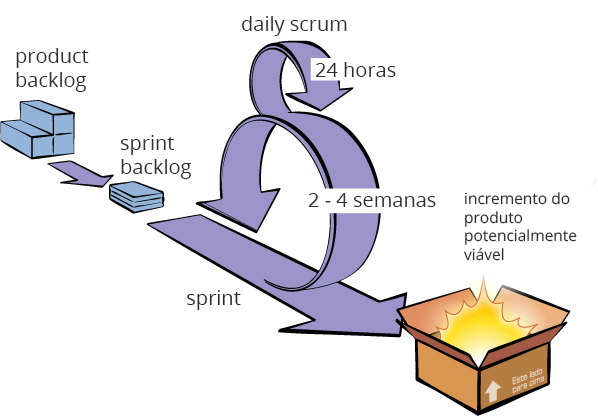
\includegraphics[width=1\textwidth]{images/ciclos_scrum.jpg}
\caption{Ciclo do Scrum. }
\label{fig:cicloscrum}
{\small Fonte: http://www.desenvolvimentoagil.com.br/scrum. Acessado em: 01/02/2017} %Fonte da imagem
\end{figure}


%TODO completar a frase (done!)

O método mais eficiente e eficaz de transmitir informação para e dentro de uma equipe de desenvolvimento é a conversa face-a-face. Tratando-se da experiência do usuário, surgiu o conceito de \textit{Lean UX}, que é o desenvolvimento ágil focado no usuário.

O \textit{Lean UX} é definido como uma abordagem para um desenvolvimento de software centrado no usuário, especialmente em \textit{startups}, criando produtos radicalmente novos. Ele tenta romper com os silos organizacionais e ciclos de produção como, por exemplo, o processo de desenvolvimento de software em cascata \cite{Liikkanen:2014:LUN:2639189.2670285}. 

São identificadas três principais influências no \textit{Lean UX}: movimento \textit{design thinking}, método \textit{Learn startup} e desenvolvimento de software ágil \cite{gothelf2013lean}.

O \textit{design thinking} é importante para o \textit{Lean UX} pois toma a posição explícita de que todos os aspectos de um negócio podem ser abordados com métodos de design. O pensamento de design é uma fundação crítica que incentiva as equipes a colaborar entre papéis e considerar o design do produto de uma perspectiva holística \cite{robbinsd:beck2001agile}.

A \textit{Lean Startup} defende a criação de protótipos rápidos projetados para testar as premissas do mercado e usa o \textit{feedback} dos clientes para evoluí-los muito mais rápido do que as práticas de engenharia de software tradicionais \cite{robbinsd:beck2001agile}. Esse método aumenta a frequência de contato com os clientes e minimizam o risco de entregas atrasadas do projeto e faz com que a equipe desenvolva mais rapidamente.

\section{Desenvolvimento front-end}
O desenvolvimento \textit{front-end} está relacionado a aspectos visuais e é onde o usuário interage com a aplicação diretamente, para que o \textit{back-end} - linguagens de programação - possa processar esses dados. Durante o desenvolvimento \textit{front-end}, muito se foi pensando na responsividade das páginas.

O web design responsivo é uma abordagem de desenvolvimento web que cria alterações dinâmicas na aparência de um site, dependendo do tamanho da tela e da orientação do dispositivo usado para visualizá-lo \cite{ResponsiveWebDesignNNG}.

Com a utilização de padrões web como HTML5, CSS e Javascript, ou do \textit{framework} Bootstrap, é possível desenvolver páginas web responsivas que podem adaptar a arquitetura da informação de uma página em qualquer tamanho e resolução de tela.

Por meio de um layout fluido, conteúdo flexível e de padrões web que podem  detectar capacidades de tamanho de tela, resolução, densidade de pixel e orientação, desenvolvedores podem criar contextos e adaptáveis \cite{Responsive}.

O HTML (Linguagem de Marcação de Hypertexto, do inglês HyperText Markup Language) é uma linguagem que descreve o conteúdo de documentos web \cite{html5}. Na sua versão 5, possui características que tornam fáceis o trabalho com multimídias e gráfica, sem recorrer a plugins e APIs de terceiros.

O CSS (Folha de estilo em cascata, do inglês \textit{Cascate Style Sheet}) é uma linguagem que descreve o estilo de um documento HTML. O CSS, atualmente na versão 3, formata a informação entregue pelo HTML. Essa informação pode ser imagem, fontes, texto, vídeo, áudio ou qualquer outro elemento criado \cite{css3}. Ele permite adaptar a apresentação da informação em diferentes tipos de dispositivos, com tamanhos diferentes de telas e também auxilia na formatação de informações para impressão.

O Javascript (Js) é uma linguagem de programação interpretada de múltiplos paradigmas,
baseado na orientação a objetos, imperativo e declarativo \cite{javascript}. Já o Bootstrap, um \textit{framework} de código livre para desenvolvimento de projetos responsivos, que se adaptam à diferentes resoluções de tela, baseado em Javascript, assim como em HTML5 e CSS3.


\section{Análise e especificação de requisitos}

Requisito é uma afirmação sobre um produto a ser projetado, que especifica o que deve, o que não deve, ou como deve ser construído \cite{Sommerville:2010:SE:1841764}. Um dos principais objetivos do estabelecimento de requisitos é fazê-los específicos e claros. A ampla área de tarefas e técnicas que levam à compreensão dos requisitos é chamado de. engenharia de requisitos. 

A engenharia de requisitos é uma ação de engenharia de software que começa durante a atividade de comunicação e continua na atividade de modelagem. Deve ser adaptada as necessidades do processo, do projeto, do produto e das pessoas que fazem o trabalho \cite{Pressman:2001:SEP:572512}. 


\section{Prototipação}

Uma das formas mais eficazes de criar um MVP é através da prototipagem de experiência do usuário. Um protótipo é uma aproximação de uma experiência que permite simular o que é e como usar o produto ou serviço em questão necessitando, então, de ser clicável. Ao mesmo tempo, seu objetivo deve ser gastar o menor esforço possível para criar o protótipo, o que torna a escolha da ferramenta de prototipagem importante. No processo da engenharia de requisitos, o protótipo pode ajudar na elicitação e validação dos requisitos \cite{Sommerville:2010:SE:1841764}.

O \textit{wireframe} é uma representação de baixa fidelidade de uma interface. Mockup é uma representação estática de média a alta fidelidade, e protótipo é uma representação dinâmica de alta fidelidade, simulando a interface de interação com o usuário \cite{Sommerville:2010:SE:1841764}.

\subsection{Protótipo de baixa fidelidade}

Os protótipos de baixa fidelidade podem ser feitos dos componentes mais acessíveis como papel, canetas, permitindo simular experiências de uma maneira rápida. Nenhum investimento é necessário e permite a equipe um senso de como o produto deve funcionar \cite{Sommerville:2010:SE:1841764}.

\subsection{Protótipo de alta fidelidade}
Os protótipos de alta e média fidelidade têm significativamente mais detalhes do que os protótipos baseados em \textit{wireframes}. Pode-se utilizá-los para demonstrar e testar projetos que são desenvolvidos com um nível de interação semelhante da experiência do produto final \cite{Sommerville:2010:SE:1841764}.


\section{Avaliação Heurística}
% TODO - é importante descrever aqui o que é uma avaliação heurística, como é feita, em termos conceituais, já que você utilizou no projeto (done!)

A avaliação heurística é um método informal para a análise da usabilidade e é realizada inspecionando uma interface, e tentando chegar a uma opinião sobre o que é bom e ruim sobre ela. Tem como vantagem ser barata, intuitiva e fácil de motivar as pessoas a fazê-la. Ela não requer um planejamento avançado, e pode ser usado claramente no desenvolvimento de processos. Como desvantagem, este método, às vezes, identifica problemas de usabilidade sem prover sugestões diretas em como resolvê-los ~\cite{Nielsen:1990:HEU:97243.97281}.

Ela tem como objetivo encontrar problemas de usabilidade em designs de interface de usuário, com um pequeno número de avaliadores que examinam e julgam uma interface e suas complicações, com base nos princípios de usabilidade \cite{Nielsen:1992:FUP:142750.142834}.


Cada participante classifica o problema a um fator de gravidade de acordo com as severidades propostas por \cite{severidades}, considerando a influência dos problemas na realização das atividades. A classificação das severidades ajudam a fornecer uma estimativa aproximada da necessidade de esforços adicionais de usabilidade. As cinco severidades são:

  
0 = Não acredito que seja um problema

1 = Cosmético: Não há necessidade imediata de solução

2 = Pequeno: Problema de baixa prioridade

3 = Grande: Problema de alta prioridade

4 = Catástrofe: Problema muito grave, deve ser reparado imediatamente


Na avaliação heurística colaborativa, cada participante é livre para indicar um problema na interface.  Ao final da avaliação, para catalogar os dados, foi realizada uma média das severidades dada pelos 5 especialistas participantes à cada problema, e atribuído, a cada um, sua(s) heurística(s) correspondente(s), segundo as 10 heurísticas propostas por Nielsen e Molich \cite{Nielsen:1990:HEU:97243.97281}:


Heurística 1 - Visibilidade do status do sistema: O sistema deve sempre manter os usuários informados sobre o que está acontecendo, através de feedback adequado dentro de um prazo razoável.

Heurística 2 - Correspondência entre o sistema e o mundo real: O sistema deve falar o idioma dos usuários, com palavras, frases e conceitos familiares para o usuário, em vez de termos orientados ao sistema. Siga as convenções do mundo real, fazendo com que as informações apareçam em uma ordem natural e lógica.


Heurística 3 - Controle do usuário e liberdade: Os usuários muitas vezes escolhem funções do sistema por engano e precisarão de uma "saída de emergência" claramente marcada para deixar o estado indesejado sem ter que passar por um diálogo estendido. Suporte desfazer e refazer.

Heurística 4 -  Consistência e padrões: Os usuários não devem ter que se perguntar se diferentes palavras, situações ou ações significam a mesma coisa. Siga as convenções da plataforma.

Heurística 5 - Prevenção de erros: Melhor do que boas mensagens de erro é um design cuidadoso que impede que um problema ocorra em primeiro lugar. Elimine as condições propensas a erros ou procure por elas, e apresente aos usuários uma opção de confirmação antes de se comprometerem com a ação.

Heurística 6 - Reconhecimento em vez de recordação: Minimize a carga de memória do usuário, tornando visíveis objetos, ações e opções. O usuário não deve se lembrar de informações de uma parte do diálogo para outra. As instruções de utilização do sistema devem ser visíveis ou facilmente recuperáveis sempre que adequado.        

Heurística 7 - Flexibilidade e eficiência de utilização: Aceleradores - invisível pelo usuário novato - muitas vezes pode acelerar a interação para o usuário especializado, de tal forma que o sistema pode servir tanto para usuários inexperientes e experientes. Permita que os usuários adaptem ações frequentes.  

Heurística 8 -  Estética e design minimalista: Os diálogos não devem conter informações irrelevantes ou raramente necessárias. Cada unidade extra de informação em um diálogo compete com as unidades relevantes de informação e diminui sua visibilidade relativa.     


Heurística 9 - Ajude os usuários a reconhecer, diagnosticar e resolver erros:  Mensagens de erros devem ser expressas em linguagem clara (sem códigos), indicar com precisão o problema e construtivamente sugerir uma solução.

Heurística 10 - Ajuda e documentação: Mesmo que seja melhor que um sistema pudesse ser usado sem documentação, pode ser necessário fornecer uma ajuda e documentação. Qualquer informação deve ser fácil de ser pesquisada, com foco na atividade do usuário, lista de passos concretos a serem realizados, e não ser muito grande.   




\chapter{ATIVIDADES DESENVOLVIDAS}

Este capítulo descreve as atividades que foram realizadas no projeto desenvolvido durante o estágio. O estagiário realizou 352 horas de estágio, no período de 23 de maio a 02 de setembro de 2016.

\section{Ambientação e treinamento}
Durante as primeiras semanas do estágio, houve um período de ambientação sobre os projetos desenvolvidos na empresa, metodologias utilizadas e ferramentas. 

Durante a ambientação, o estagiário fez treinamento de Git\footnote{https://git-scm.com}, um sistema de controle de versão distribuído, e um sistema de gerenciamento de código fonte, com ênfase em velocidade. 

As atividades inicias foram focadas em atualizações e melhorias dos portais da empresa.

\section{Desenvolvimento front-end}
Simultaneamente aos trabalhos no projeto do software de planejamento estratégico, demandas de front-end surgiram, principalmente na criação de portais e manutenção dos existentes. A atuação como desenvolvedor front-end possibilitou a utilização das linguagens HTML5, CSS3, Javascript e o framework Bootstrap para a criação e manutenção de soluções online.

Um dos websites desenvolvidos foi o portal de apresentação do software. Foi desenvolvido utilizando as linguagens HTML5, CSS3, Javascript, Bootstrap e Hightcharts. O processo de desenvolvimento consistiu em levantamento de requisitos, formulação de conteúdo, prototipação, implementação e testes. O objetivo do portal é apresentar o software de uma forma clara e concisa, apresentando o projeto, as instituições participantes e estatísticas de pesquisas, em uma página de conversão única chamada ladingpage. Para a demonstração de dados coletados no desenvolvimento do projeto em forma de gráficos, foi necessário a utilização do framework Highcharts.

O Highcharts\footnote{http://www.highcharts.com} é um software de criação de web gráficos que produz gráficos animados utilizando JavaScript e HTML5 SVG. Ele funciona em todos os navegadores modernos e é exclusivamente com base em tecnologias de navegador nativo, isto é, não requer a instalação de plugins e extensões como Flash ou Java.


\section{Análise e especificação de requisitos}
Os requisitos do software eram coletados em reuniões com o cliente. Esses dados eram estudados e discutidos pela equipe e a especificação era realizada, através de documentações e protótipos.

Durante todas as etapas de desenvolvimento, os gestores do projeto, que também utilizarão o sistema no futuro, acompanhavam e homologavam as especificações e os protótipos desenvolvidos.

\section{Prototipação}

% TODO - a parte dos conceitos deveria ir para o capítulo anterior - aqui você descrever como foi a sua atividade***done!

Durante todo o desenvolvimento do software, os wireframes, mockups e protótipos foram criados para serem validados junto ao cliente e, ao mesmo tempo, sendo uma referência útil à equipe de programadores.

Após a análise e especificação, os protótipos ajudam a ter a primeira noção de como o sistema irá se parecer. Os protótipos serviram para os clientes validarem o que a equipe de especificação e design especificaram e, também, aos desenvolvedores, ajudando no momento da implementação. Os protótipos são uma aproximação de uma experiência que permite o usuário fazer uma simulação de como o produto em questão será.

Inicialmente, os protótipos foram baseados em wireframes e mockups, com o objetivo de demonstrar como os dados ficariam organizadas na interface.  

Um grande aprendizado durante a elaboração dos protótipos foi a de especificar as telas com dados que reaproximassem de dados reais. Isso permitiu ter uma abordagem mais concisa sobre os dados e, além disso, facilitava a homologação.

\subsection{Protótipo de baixa fidelidade}

O wireframe, como representa a Figura \ref{fig:wireframe} é uma representação de baixa fidelidade de uma interface. Foi reproduzido digitalmente.

\begin{figure}[H]
\centering
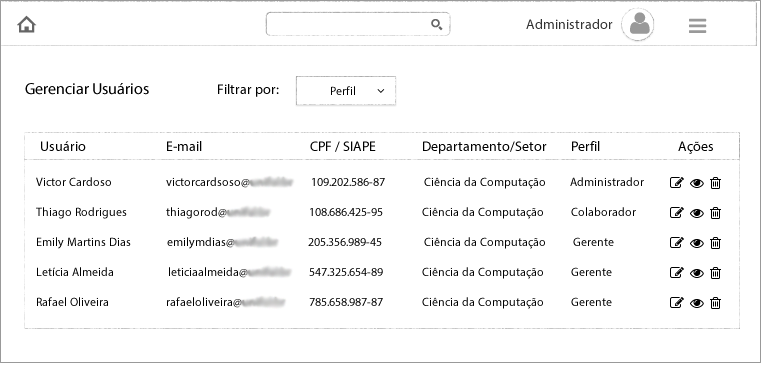
\includegraphics[width=1\textwidth]{images/wireframe.png}
\caption{Wireframe inicial}
\label{fig:wireframe}
\end{figure}

\subsection{Protótipo de alta fidelidade}
O mockup é uma representação estática do design próximo ao produto final. O design do software passou por várias modificações até encontrar, juntamente com o cliente, a melhor solução para a disposição dos dados na interface. A Figura \ref{fig:dashboard0} mostra a primeira versão do Painel de bordo do sistema, local onde os dados são apresentados em forma de tabelas e gráficos. Assim como a Figura \ref{fig:dashboard0_1} apresenta uma variação do mockup após sugestões do cliente. 

\begin{figure}[H]
\centering
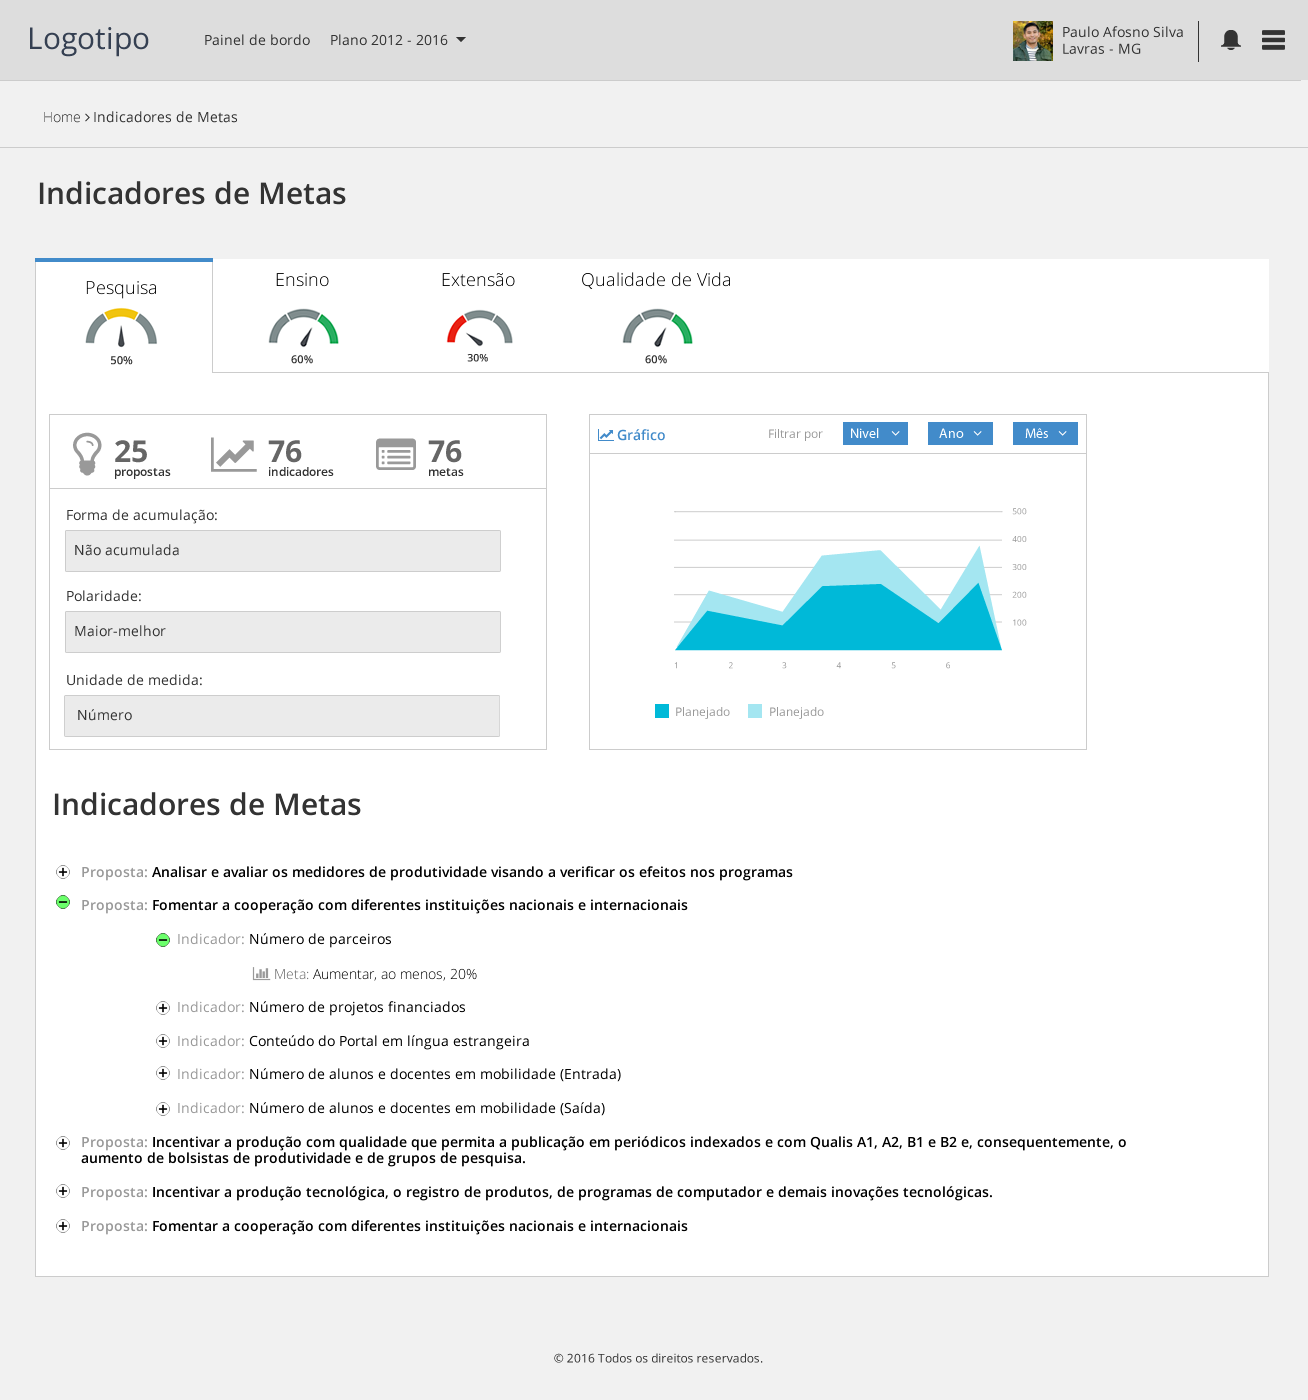
\includegraphics[width=1\textwidth]{images/dashboard0.png}
\caption{Mockup inicial}
\label{fig:dashboard0}
\end{figure}


\begin{figure}[H]
\centering
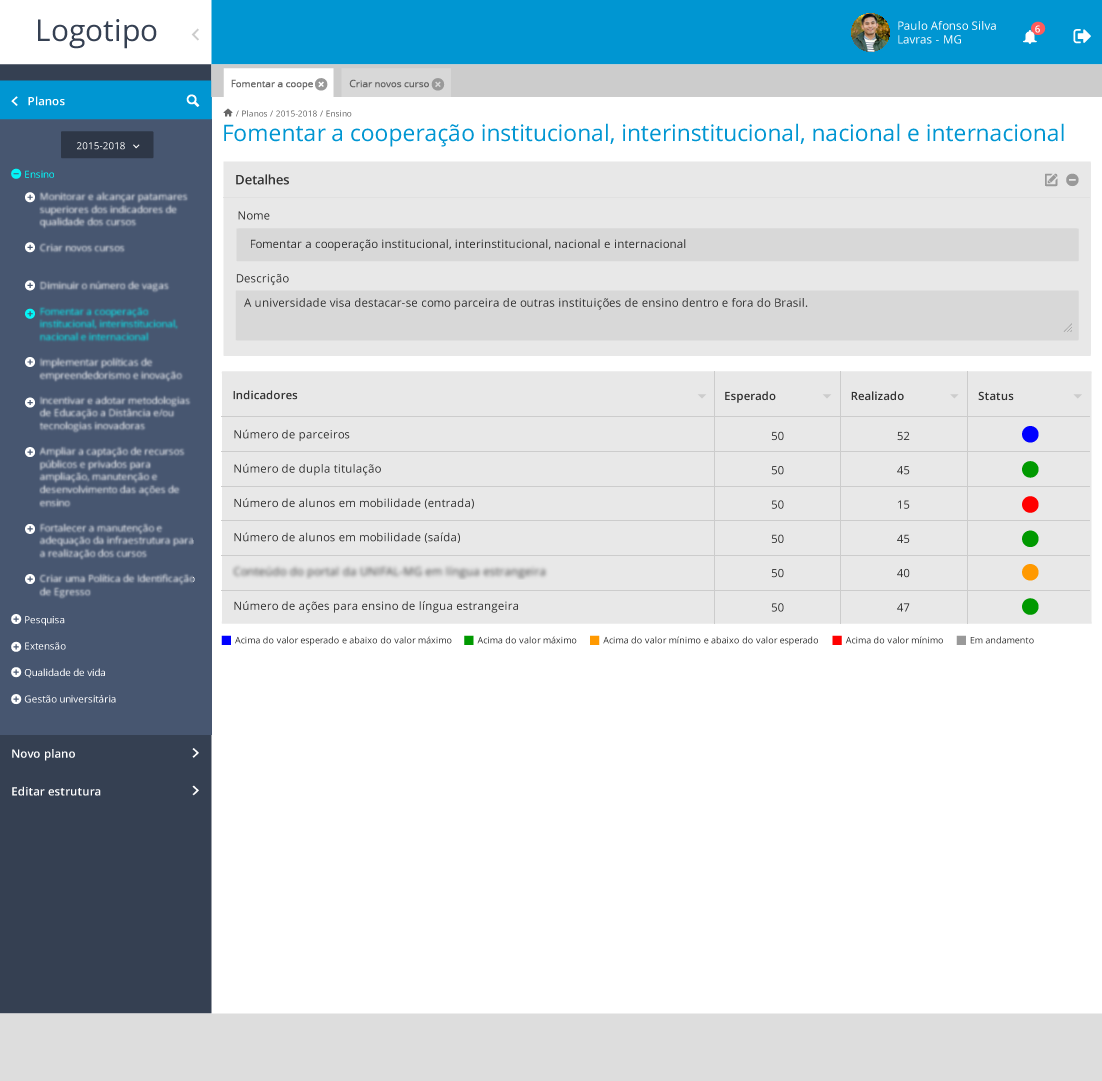
\includegraphics[width=1\textwidth]{images/dashboard0_1.png}
\caption{Segunda versão do mockup inicial}
\label{fig:dashboard0_1}
\end{figure}



Após uma série de ciclos, encontrou-se a melhor solução para o painel de bordo, utilizando um design limpo e com informações que seriam relevantes ao usuário.

%Informações removidas por serem confidenciais

% As Figuras \ref{fig:mockup11} e \ref{fig:mockup2} representam os mockups após estudos de viabilidade, modificações e reuniões com os clientes.

%\begin{figure}[H]
%\centering
%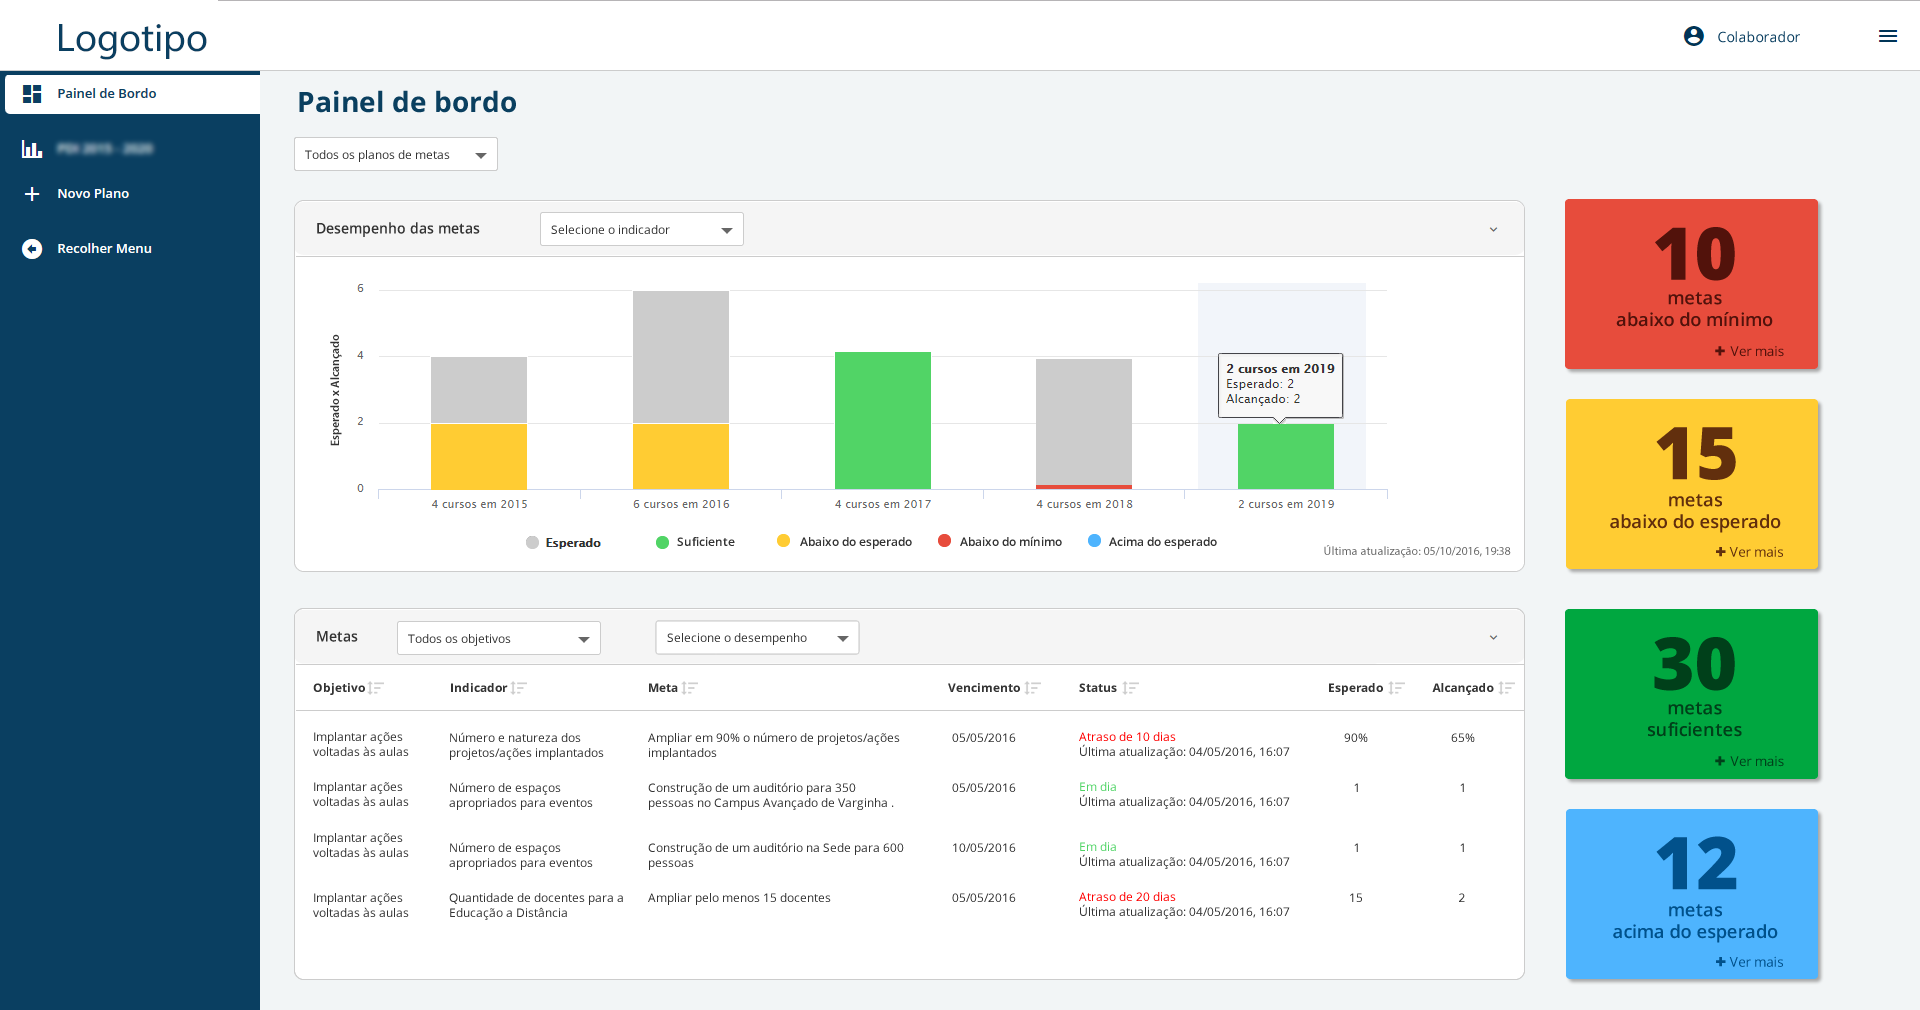
\includegraphics[width=1\textwidth]{images/mockup1.png}
%\caption{Mockup do Painel de bordo}
%\label{fig:mockup11}
%\end{figure}

%\begin{figure}[H]
%\centering
%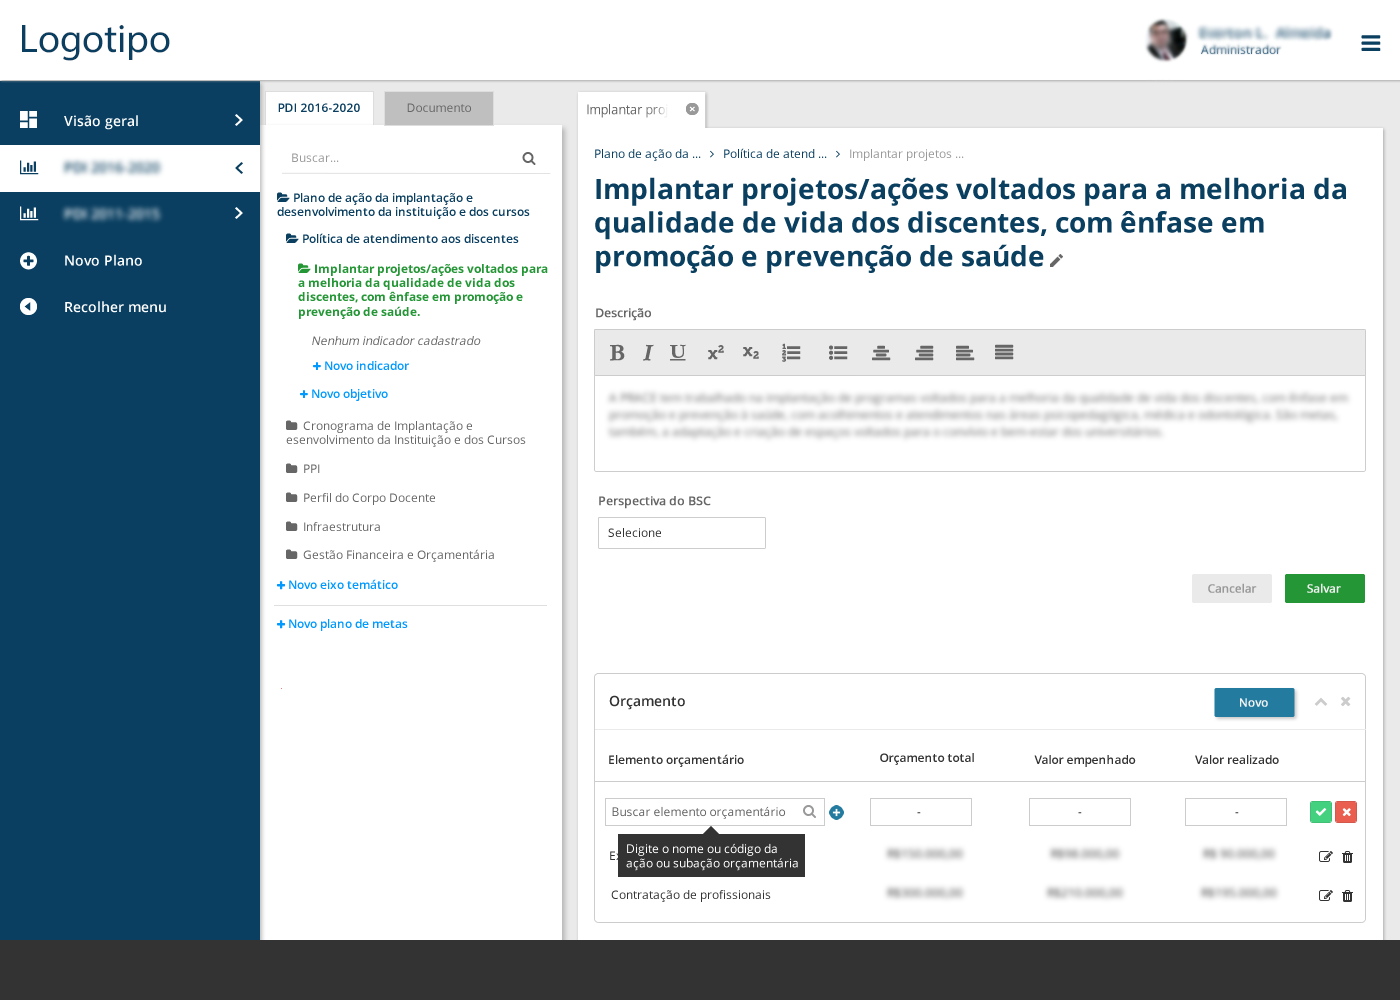
\includegraphics[width=1\textwidth]{images/mockup2.png}
%\caption{Mockup da estrutura}
%\label{fig:mockup2}
%\end{figure}

\subsection{Ferramentas utilizadas}
Os mockups e os wireframes foram desenvolvidos utilizando três softwares de manipulação de imagens diferentes, Adobe Photoshop versão CC, Adobe Fireworks versão CS6 e Adobe Illustrator versão CC. Para os protótipos dinâmicos, utilizou-se as ferramentas    MarvelApp e Axure versão RP.

\subsubsection{Adobe Illustrator}
O Adobe Illustrator\footnote{http://www.adobe.com/br/products/illustrator.html} é um editor de imagens vetoriais desenvolvido e comercializado pela Adobe Systems. Foi criado inicialmente para o Apple Macintosh em 1985 como complemento comercial de software de fontes da Adobe e da tecnologia PostScript desenvolvida pela empresa. Ele permite o desenvolvimento de imagens vetoriais.

\subsubsection{Adobe Photoshop}
O Adobe Photoshop\footnote{http://www.adobe.com/br/products/photoshop.html} é um software caracterizado como editor de imagens bidimensionais do tipo raster (possuindo ainda algumas capacidades de edição típicas dos editores, como Illustrator) desenvolvido pela Adobe Systems. É considerado o líder no mercado dos editores de imagem profissionais. Sua mais recente versão é o Adobe Photoshop CC, sua décima quarta edição 14.0

\subsubsection{Adobe Fireworks}
O Fireworks\footnote{http://www.adobe.com/br/products/fireworks.html} é um editor de imagens de bitmap e desenho vetorial desenvolvido pela Macromedia, posteriormente adquirido pela Adobe. Suas funcionalidades focam a publicação gráfica na Internet, por isso inclui suporte a GIF animado, PNG e imagens fatiadas, além de possuir ótima compressão de imagens. 

\subsubsection{MarvelApp}
 O MarvelApp\footnote{https://marvelapp.com} permite a criação de protótipos de alta fidelidade de maneira rápida, eficiente e portátil para testes realizados em smartphones. A partir de imagens e mockups, é possível transformá-los em protótipos para qualquer tipo de dispositivo, sem necessidade de codificação.

\subsubsection{Axure}
Soluções podem ser prototipadas e validadas pelas pessoas que melhor compreendem seus negócios, produtos e clientes. O Axure\footnote{https://www.axure.com} permite a criação de flowcharts, wireframes, mockups, personas e quadro de ideias. Além disso, permite uma maior interação juntamente com a entrada de dados pelo usuário.

\section{Desenvolvimento ágil}
Durante o desenvolvimento do projeto, foi utilizado o Trello\footnote{https://trello.com/} (Figura \ref{fig:trello}) como gerenciador de atividades da equipe. O Trello é um aplicativo de gerenciamento de projeto baseado na web, utilizando o paradigma Kanban para gerenciamento de projetos. Utilizando o Trello no projeto, as \textit{sprints} foram representadas pelos quadros (\textit{boards}), que contêm atividades. As atividades são representadas por cartões que são criados dentro dos quadros. Cada atividade é subdivida em tarefas, como um \textit{checklist}. No caso de especificação, as tarefas eram dividias em análise, especificação, design de interface e prototipação. Como vantagem, é possível representar o progresso da atividade, desta forma, a equipe tinha uma visão das atividades de todos, facilitando a comunicação.

As \textit{sprints} duravam de uma a três semanas, sendo que a duração mais comum era de duas semanas. No início de cada \textit{sprint}, a equipe se reunia para a reunião de \textit{planning}, onde as próximas atividades são apresentadas e a equipe divide as atividades em tarefas e estima quantas horas serão gastas para cada atividade. Durante o \textit{sprint}, havia reuniões diárias, chamadas de \textit{standup meeting} (reunião em pé, com o objetivo de serem rápidas), para cada membro da equipe falar o que foi desenvolvido, quais suas dificuldades e o que será desenvolvido posteriormente. E, ao final do \textit{sprint}, eram realizadas as reuniões de \textit{review} e \textit{retrospective}, para analisar se o objetivo do \textit{sprint} foi alcançado, e levantar os pontos fortes, pontos fracos e melhorias futuras. 

Observou-se que, ao utilizar essa metodologia durante o projeto, a comunicação entre os membros da equipe foi beneficiada e todos puderam ter uma noção do trabalho que estava sendo desenvolvido pelos outros. Outro fator importante a ser destacado foi a possibilidade de trabalho em conjunto das equipes de especificação, desenvolvimento e testes.

\begin{figure}[H]
\centering
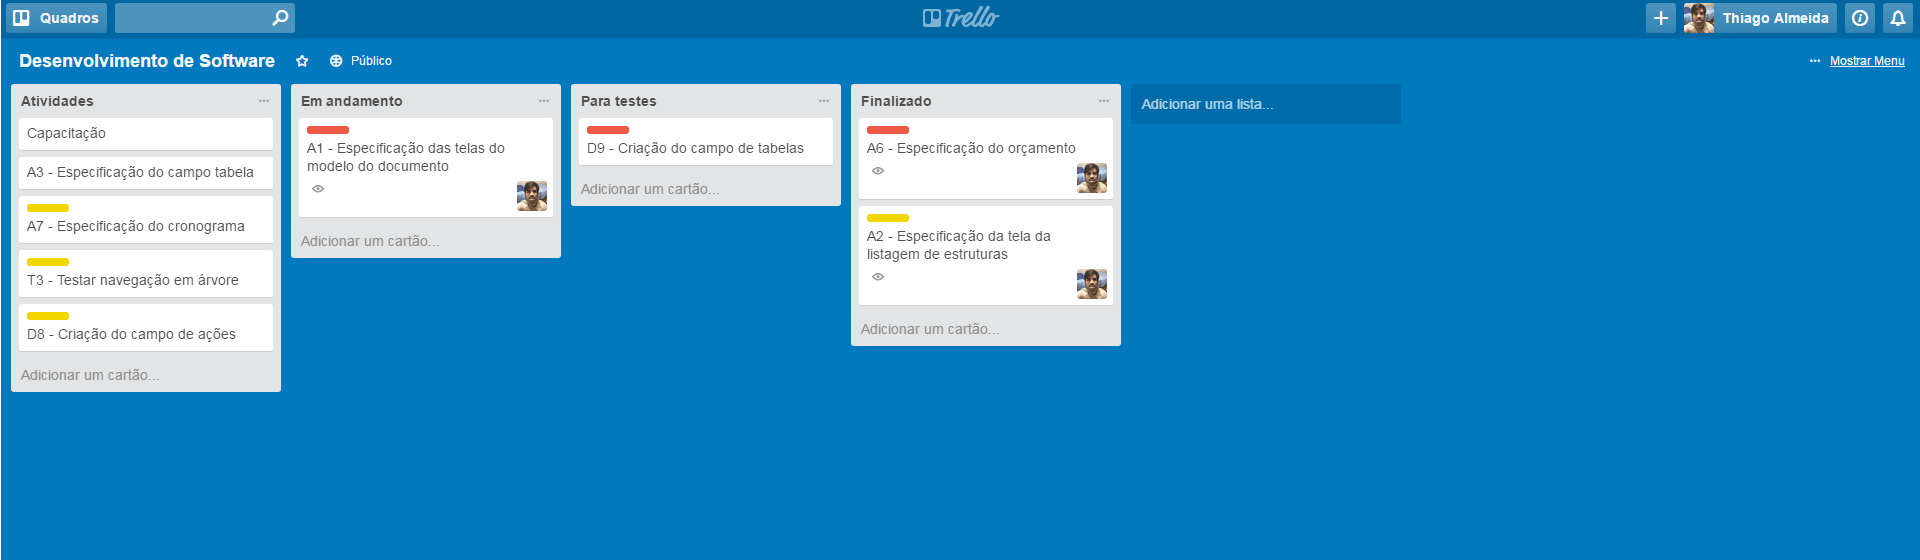
\includegraphics[width=1\textwidth]{images/trello.png}
\caption{Gerenciador de atividades - Trello }
\label{fig:trello}
\end{figure}


%\subsection{GitHub}
%GitHub é um serviço de Web Hosting Compartilhado para projetos que usam o controle de versionamento. Ele oferece funcionalidades como envio de código e correções, versionamento, issue tracker, entre outros.


%\section{personas}

%Foram consideradas personas do ForPDI  gestores, técnicos administrativos e professores de instituições federais de ensino superior. Os principais usuários do sistema serão os responsáveis pelo planejamento, elaboração, execução e acompanhamento do PDI da instituição de ensino. Haverá também a possibilidade da comunidade acessar alguns dados do sistema, acompanhando o andamento do PDI da instituição referente.

\section{Avaliação Heurística}

Foi realizada a avaliação heurística do software de planejamento estratégico na forma colaborativa, em duas sessões de 2 horas cada, com a participação de 5 especialistas em usabilidade. Sobre isso, Nielsen e Molich  \cite{Nielsen:1990:HEU:97243.97281} afirmam que os resultados de uma avaliação heurística serão muito melhores se houver várias pessoas conduzindo a avaliação, fazendo-a independentemente uns dos outros, e recomenda que a avaliação heurística seja feita com entre três e cinco avaliadores. A avaliação foi realizada em duas sessões, de aproximadamente 2 horas cada.
 

Foram consolidadas 5 tarefas a serem realizadas:

\begin{itemize}
\item login no sistema: nesta tarefa espera-se que o usuário realize o login no sistema (Obrigatório), recupere sua senha;
\item cadastro de domínio: nesta tarefa espera-se que o usuário cadastra o domínio;
\item cadastro de estrutura: nesta tarefa, espera-se que o usuário cadastre uma nova estrutura;
\item cadastro de plano estratégico: espera-se que o usuário cadastre um novo plano estratégico macro;
\item cadastro de plano de metas: nesta tarefa, espera-se que o usuário cadastre um novo plano de metas, cadastrando todo o fluxo de níveis,  a partir de um plano já cadastrado anteriormente. Será entregue um papel com as informações que devem ser inseridas em cada nível.
\end{itemize}

\subsection{Resultados}

Como resultado, obteve-se uma lista de problemas identificados, juntamente com as heurísticas afetadas, graus de severidade e, em muitos dos problemas, soluções propostas pelos avaliadores.

A partir da análise da avaliação heurística com especialistas da área, foram encontrados 118 problemas de usabilidade. Os dados referentes às violações categorizadas por severidade podem ser visualizados na Tabela ~\ref{tab:severidade}. A maioria dos problemas (83,78\%) foram classificados pelos avaliadores como problemas com severidade Simples (2). Em segundo lugar, com 41,3\%, foram classificados os problemas com severidade Sério (3). 

\begin{table}[H]
\centering
\caption{Severidades}
\label{tab:severidade}
\begin{tabular}{c|c|c}
      \hline
       \rowcolor[gray]{.9}
      \bf Severidade  & \bf Frequência & \bf Porcentagem  \\
      \hline
      \hline
0 (Não acredito que seja um problema) & 0          & 0\%         \\
1 (Cosmético)                        & 12         & 14,16\%     \\
2 (Simples)                          & 71         & 83,78\%     \\
3 (Sério)                           & 35         & 41,3\%      \\
4 (Catastrófico)                     & 0          & 0\%         \\

\hline
\hline
\bf TOTAL   & \bf 118        & \bf 100\%   \\
 \hline 
\end{tabular}
\end{table}



Entre os principais problemas elencados, destaca-se os relacionados a falta de \textit{feedback} e ajuda para o usuário. Não havia algum manual ou indicador de localização para que o usuário possa identificar o local onde está e o que deve fazer. Havia falta de \textit{feedbacks} quando o usuário realizava alguma ação no sistema, mesmo que a ação fosse realizada com sucesso. 

\begin{table}[H]
\centering
\caption{ Violações categorizadas por Heurísticas}
\label{tab:heuristicasAfetadas}
\begin{tabular}{c|c|c}
      \hline
      \rowcolor[gray]{.9}
 \bf Heurística   &  \bf Frequência & \bf Porcentagem  \\
      \hline
      \hline
H1. Visibilidade do status do sistema
& 10  & 7\%\\

H2. Correspondência entre o sistema e o mundo real 
& 15 & 10\% \\  

H3. Controle do usuário e liberdade                     
& 9  & 6\%     \\

H4. Consistência e padrões                          
& 29  & 19\%      \\

H5. Prevenção de erros                        
&15  & 10\%      \\

H6. Reconhecimento em vez de recordação                 
&3  &2\%      \\

H7. Flexibilidade e eficiência de utilização           
&5  &3\%      \\

H8. Estética e design minimalista                       
& 21  & 14\%      \\

H9. Ajude os usuários a reconhecer, diagnosticar e resolver erros                
& 15  &10\%      \\

H10. Ajuda e documentação                       
&15  &10\%      \\


\hline
\hline
\bf TOTAL   & \bf 137        & \bf 100\%   \\
 \hline 
\end{tabular}
\end{table}

A Heurística 4, consistência e padrões, obteve a maior frequência de problemas, com 29 ocorrências, representando 21\% das violações. A segunda maior violação foi a Heurística 8, estética e design minimalista, com 21 ocorrências, representando 15\% das violações. 

Em relação aos problemas que afetam a Heurística 4, consistência e padrões, o sistema apresentou padronizações diferentes para ações iguais, como larguras e alturas diferentes para elementos com as mesmas funções, padronização de campos, como data, sem máscara ou informar ao usuário, a forma correta e botões de salvar e cancelar aparecendo em diferentes lugares em contextos semelhantes.

A Heurística 8, estética e design minimalista, está relacionado a simplicidade da interface em relação à arquitetura da informação. Problemas como contraste de cores de ícones, campos pequenos ou muito grandes, textos muito grandes que tornam a tela com muitas informações, principalmente na árvores de níveis do software, foram encontrados.

E nas Heurísticas 9 e 10, ajude os usuários a reconhecer, diagnosticar e resolver erros, e ajuda e documentação, respectivamente,  observou-se a falta de ajuda no sistema sobre o que se tem que fazer. Por se tratar de formulários com grande quantidade de campos, e alguns específicos da área de planejamento institucional, observou-se a falta de informações sobre a funcionalidade do campo a ser preenchido. O sistema também não continha informações precisas sobre erros ao submeter uma informação no sistema.


\subsection{Melhorias implantadas}
Os problemas encontrados nos testes e nas avaliações heurísticas foram cadastrados no repositório do projeto, para serem corrigidos pela equipe. Um levantamento realizado três meses após a avaliação heurística mostrou que, dos 118 problemas de usabilidade encontrados, 87 foram resolvidos, totalizando 74\% de problemas corrigidos. O resultado esperado compreendeu as expectativas da equipe e dos gestores e seguiu o planejamento inicial do projeto. 

\subsubsection{Mensagens de alerta e erro}
Foram estabelecidas mensagens de erros, alertas e confirmações de quando há alguma mudança de contexto inesperada pelo usuário. Ao clicar no botão para deletar ou cancelar alguma ação, a mensagem de confirmação é importante para evitar que o usuário tenha clicado no botão erroneamente. Ao salvar algo, a mensagem de confirmação é mostrada ao usuário, como demonstrado na Figura \ref{fig:feedback1}. Quando o usuário comete algum erro de preenchimento nos formulários, além de mostrar uma mensagem dizendo que há erros, os erros são mostrados no específico lugar que ocorreu, como demonstrado na figura \ref{fig:erros}

\begin{figure}[H]
\centering
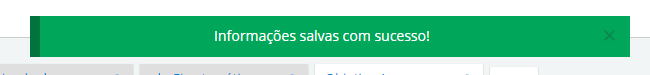
\includegraphics[width=1.1\textwidth]{images/feedback1.png}
\caption{Mensagem de confirmação}
\label{fig:feedback1}
\end{figure}

\begin{figure}[H]
\centering
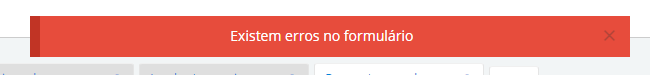
\includegraphics[width=1.1\textwidth]{images/erros.png}
\caption{Mensagem de erro}
\label{fig:erros}
\end{figure}

\subsubsection{Árvore de níveis}
A estrutura das ações, objetivos e indicadores de um planejamento estratégico é realizada por meio de níveis hierárquicos. Devido a esse fato, foi necessário desenvolver um cadastro que possibilitava o usuário visualizar qual o nível correto de cada informação. Para isso, o cadastro é realizado em forma de árvore de níveis. Após a avaliação heurística e discussão com os especialistas, a árvore foi modificada para atender melhor o usuário.

A Figura \ref{fig:arvore_geral} demonstra as três primeiras fases da evolução do design da árvore de níveis. Após estudos de viabilidade de implementação, e após a realização da avaliação heurística, a árvore foi passou por modificações, que pudessem atingir seus objetivos, com uma interface agradável ao usuário onde os dados pudessem ser organizados em forma hierárquica sem nenhuma complicação.

%Durante os ciclos de desenvolvimento, a árvore de níveis passou por modificações, como demonstrado na Figura \ref{fig:arvore_geral} que pudessem atingir seus objetivos, com uma interface agradável ao usuário. 


\begin{figure}[H]
\centering
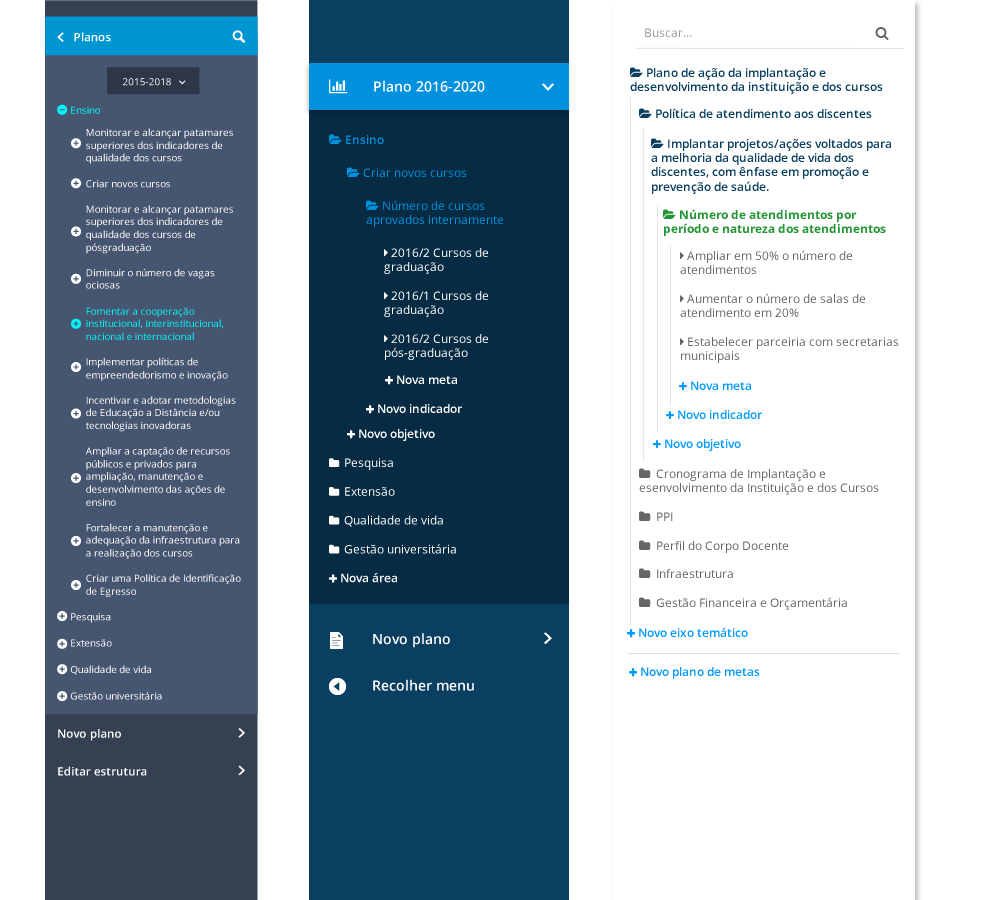
\includegraphics[width=1.1\textwidth]{images/arvore.png}
\caption{Evolução do design da árvore de níveis}
\label{fig:arvore_geral}
\end{figure}

\section{Design de interface}
Após algumas fases de análise e requisitos durante as \textit{sprints}, análises e estudos de softwares semelhantes, e avaliação heurística, o estilo de design do sistema foi estabelecido e homologado e, desde então, o software passou a ter seu estilo próprio de design, demonstrado na Figura \ref{fig:estilo}, como tamanho de fontes, tipografia, cores, formato de tabelas, gráficos e iconografia. O estilo de design permitiu o alinhamento entre as demandas de especificação e implementação. Os protótipos, que passaram a seguir o estilo de design, representavam fielmente como seria o resultado após a sua implementação. 

\begin{figure}[H]
\centering
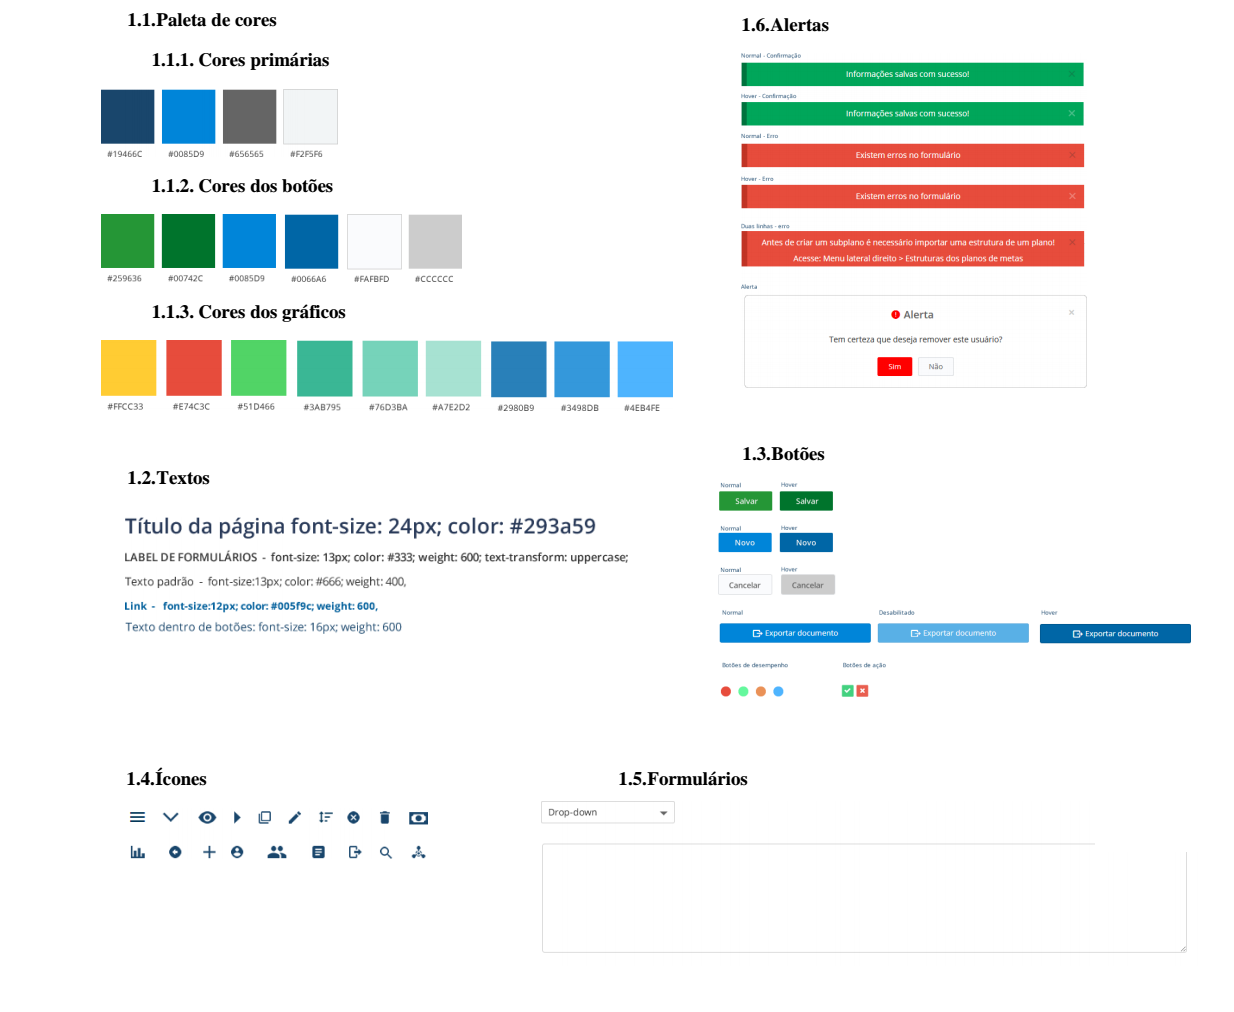
\includegraphics[width=1.1\textwidth]{images/estilo.png}
\caption{Estilo de design}
\label{fig:estilo}
\end{figure}


\section{Produto final}
\subsection{Usuários}
O software possui 4 visões de usuários diferentes, cada um com suas devidas permissões de acesso ao sistema. Para cada tipo de usuário foi pensado em um painel de bordo diferente, a fim de atender as informações relevantes àquele específico usuário. O painel de bordo representa as informações em forma visual, por meio de gráficos, tabelas e outros elementos, organizando os dados de uma forma simplificada e sob demanda às necessidades de cada usuário. Foram desenvolvidos diagramas de fluxo de trabalho, como demonstrado na Figura \ref{fig:workflow} para ajudar a entender o fluxo de navegação por parte de cada usuário.

% alterar essa figura
\begin{figure}[H]
\centering
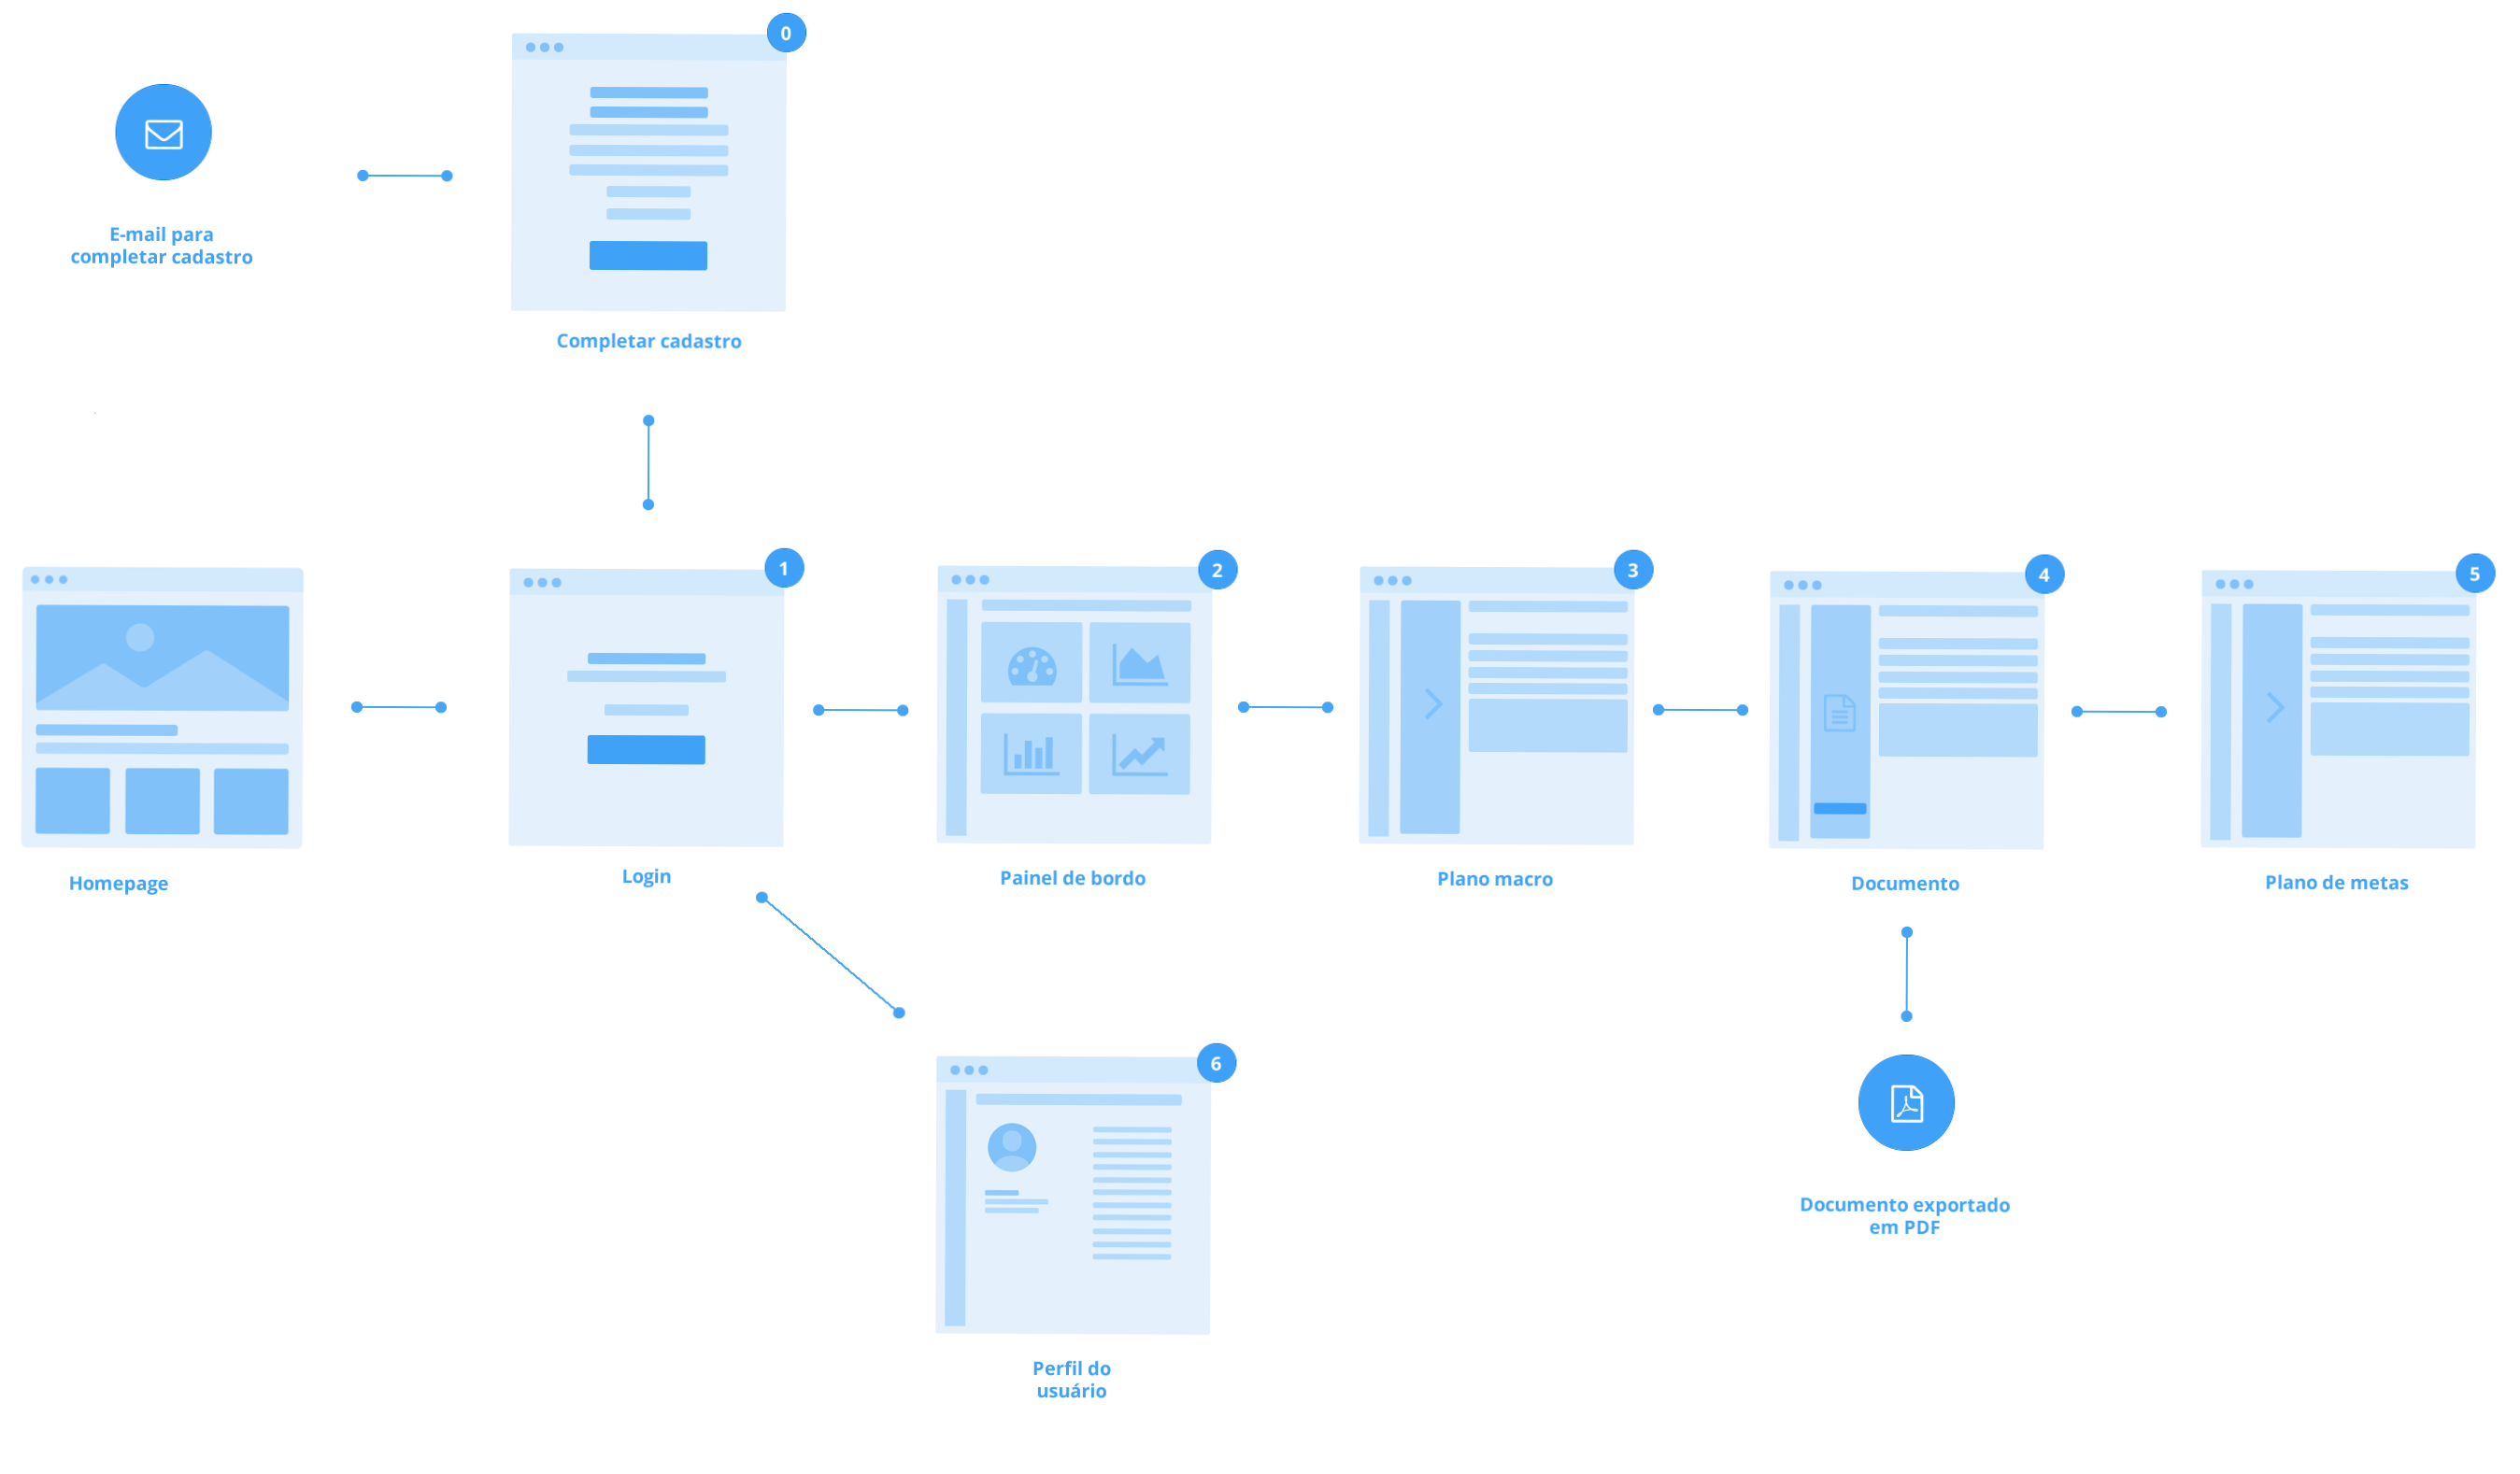
\includegraphics[width=1.1\textwidth]{images/flowwork.png}
\caption{Exemplo de diagrama de fluxo de trabalho}
\label{fig:workflow}
\end{figure}


\subsection{Estrutura dos dados}
A estrutura dos dados do planejamento estratégico é representada em níveis hierárquicos. A solução encontrada para a disposição dos dados foi em forma de árvore. Para facilitar o cadastro inicial, o usuário poderá cadastrar toda a estrutura diretamente na área da árvore do plano de metas do planejamento estratégico, com a possibilidade de editá-la no momento do cadastro ou em outro momento oportuno. 

O software possibilita importar uma estrutura do plano de metas, cada instituição ou empresa que utilizá-lo poderá torná-lo personalizado de acordo com suas estruturas de planejamento.

Após importar a estrutura, é possível cadastrar um plano macro, que contém todos os planos de metas da instituição. Cada plano de meta utiliza a estrutura importada para definir sua hierarquia. Juntamente com o plano de metas, é possível realizar a criação do documento do planejamento, e exportá-lo.


\subsection{Documento}
Ao criar um plano macro, o sistema cria uma estrutura pré-definida do documento do planejamento estratégico. A estrutura do documento é composta pelas seções e subseções seguindo o documento de referência proposto pelo cliente. A estrutura estará vazia, apenas com os títulos das seções e subseções, e os campos. O usuário poderá adicionar os campos personalizados de acordo com suas necessidades. Após o preenchimento do documento, o usuário poderá exportá-lo em formato PDF.













\chapter{CONCLUSÃO}

O estágio realizado na Progolden, como trabalho de conclusão de Curso para obtenção do título de Bacharel em Ciência da Computação, proporcionou a aplicação dos conhecimentos adquiridos no período acadêmico, em um contexto de mercado de trabalho e em um projeto de nível nacional.

O estágio proporcionou conhecimentos, tanto em nível acadêmico quanto em nível profissional. Por se tratar de uma \textit{startup} fundada por alunos e professores do Departamento de Ciência da Computação da Universidade Federal de Lavras, o estágio contribuiu para ter uma visão de como todas as áreas da empresa se relacionam e como a empresa surgiu, a partir de ideias desenvolvidas dentro da própria universidade.

%tirar essa parte do plano de desenvolvimento institucional
A participação no projeto de planejamento estratégico possibilitou experiência de desenvolver um produto, no caso, um software, desde sua concepção até a entrega. 

Os conhecimentos adquiridos na disciplina Engenharia de software ajudaram na realização das atividades de levantamento de requisitos, análise de sistemas e documentações do software.

As disciplinas Algoritmos e estruturas de dados e Banco de dados proporcionaram uma base para o desenvolvimento web e a lógica de programação, além de ajudar o estagiário no entendimento completo do software e na correção de problemas encontrados.

Os conhecimentos da disciplina Interface Homem-máquina, como design centrado no usuário, usabilidade e avaliação heurística foram aplicados durante o estágio, possibilitando o estagiário praticar metodologias que serão importantes no mercado de trabalho.

%ta mais pra médio porte kkk
A participação no projeto trouxe conhecimento para a gerência de projetos, como a divisão de atividades entre os membros e prazos de entrega, e a possibilidade de trabalhar em um projeto utilizando metodologias ágeis.

É comum que, durante as disciplinas, o aluno fique atrelado à parte conceitual e teórica, e muitas das vezes, não sabe ou encontra uma alternativa de como utilizá-las na prática. Como por exemplo, a utilização de versionamento de código, uma abordagem empregada pela maioria das empresas de desenvolvimento de software e que, durante o curso, é visto apenas na teoria, em sala de aula. A prática pôde ser exercida durante a realização do estágio.

%ta falando que é pras universidades ?
O estágio mostrou como o curso de Ciência da Computação pode contribuir na resolução de problemas do cotidiano, no caso, a falta de um software de planejamento estratégico que pudesse agilizar o trabalho de entidades organizacionais e empresas. A partir da problemática, a solução foi construída com foco no usuário e em suas reais necessidades.

Ver como a tecnologia pode influenciar, estimular e facilitar os procedimentos sobre outras áreas do conhecimento é uma motivação tamanha para continuar os estudos na área de Ciência da Computação. 

\section{Trabalhos futuros}

Como trabalho futuro, é importante a realização de testes de usabilidade com usuários reais, para que seja possível encontrar os pontos fracos e ajustá-los de acordo com as necessidades, alinhando a entrega com uma usabilidade eficiente. Com o surgimento de novos módulos e funcionalidades do software, é importante realizar novas avaliações heurísticas.

%==============================================================================
% Incluindo bibliografia
%\bibliographystyle{plain}             % estilo para labels em numeros
%\bibliographystyle{alpha}             % estilo para labels em iniciais
\bibliographystyle{abntex2-alf}           % estilo para referências usando ABNT, 
                                       % precisa instalar o abntex para usar!!!

%inclui Referências Bibliográficas
%inclui Referências Bibliográficas
\referencias
\bibliography{refbib}			% arquivo exemplo refbib.bib
%==============================================================================
% Incluindo anexos num1erados com letras maiusculas.
%\apendices
\apendice{Certificado de realização do estágio}
\label{cap:certificado}

\begin{figure}[H]
\centering
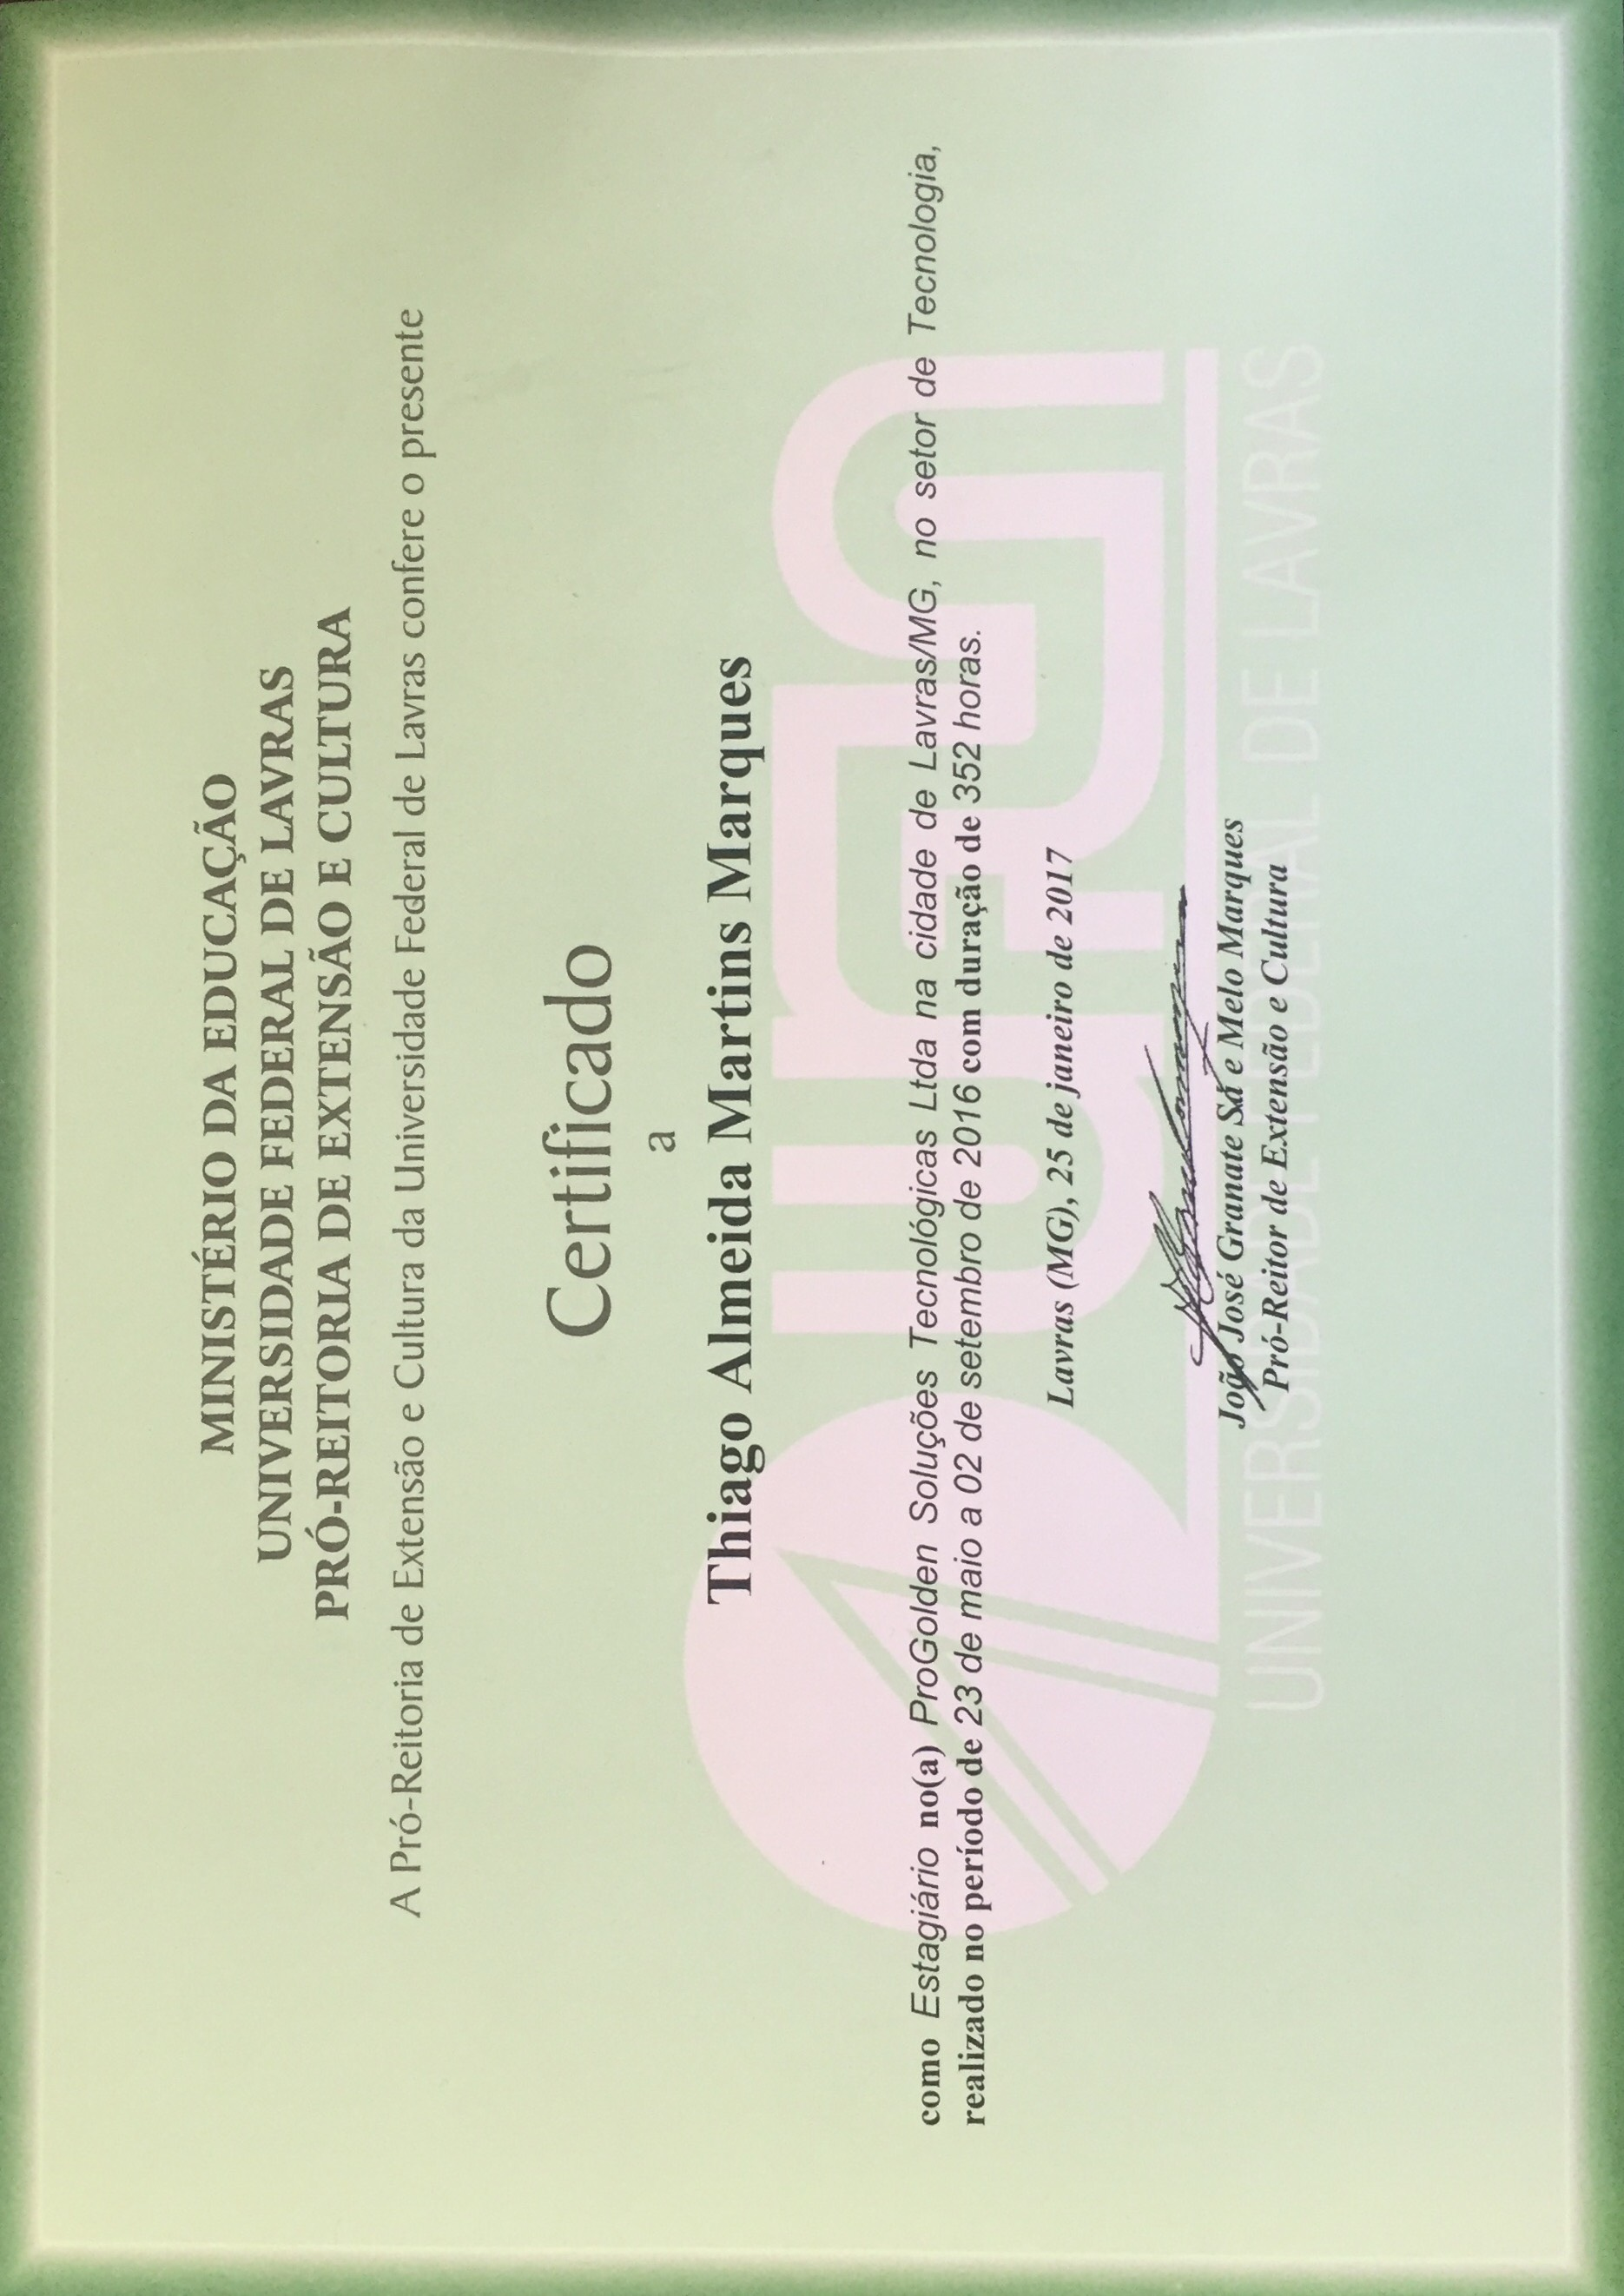
\includegraphics[width=1\textwidth]{images/certificado.JPG}
\caption{Certificado}
\label{fig:mockup1}
\end{figure}


%==============================================================================
% Fim do texto
\end{document}
